\documentclass[a4paper,11pt]{article}
\usepackage{template}
\usepackage[
  backend=biber,
  style=authoryear,
  citestyle=authoryear,
  sorting=nyt,
  url=false,
  maxnames=5,
  minnames=1,
  natbib=true
]{biblatex}
\addbibresource{olist_negative_sentiment_geometry_references.bib}
\defbibheading{bibliography}{}
\usepackage{xcolor}
\usepackage{amsmath,amssymb}
\usepackage{microtype}
\usepackage{flafter}
\usepackage[section]{placeins}

% Two-column readability tuning (Overleaf: Multiple columns / Column separation)
\setlength{\columnsep}{0.8cm}
\setlength{\columnseprule}{0pt}
\setlength{\emergencystretch}{2em}
\setlength{\tabcolsep}{4pt}
% Keep two-column body compact enough to avoid overflow from the base template.
\captionsetup{font=small}
% Optional subtle separator rule between columns:
% \setlength{\columnseprule}{0.2pt}
% \def\columnseprulecolor{\color{black!35}}

\newcommand{\fillin}[1]{\textcolor{red}{[FILL: #1]}}
\newcommand{\rqone}{When native Brazilian Portuguese e-commerce reviews are mapped into embedding space, do negative sentiments converge into distinct geometric islands, or are they diffusely distributed as a modifying layer across emergent service topic clusters?}
\newcommand{\rqtwo}{How does the degree of negative islandisation differ across Native (BERTimbau), Multilingual (MiniLM), and Cross-modal (OpenCLIP) embedding models?}

\begin{document}

\begin{titlepage}
\centering
{\Large Università degli Studi di Milano Statale\par}
\vspace{1.5cm}
{\LARGE\bfseries Geometric Analysis of Negative Sentiment in Ecommerce Reviews Across Embedding Models\par}
\vspace{1.5cm}
{\large Tram Anh Hoang\par}
{\large ID: 83447A | MA - Data Science in Economics\par}
\vfill
{\large Academic Year 2025/2026\par}
\end{titlepage}
\clearpage
\section*{AI Usage Statement}
\noindent Parts of this project were developed with the assistance of OpenAI's ChatGPT (GPT-5). The AI was used to support idea development, methodological structuring, drafting of project skeleton, and identification of relevant datasets and references.

\noindent All AI-assisted content was critically reviewed, edited, and validated by the author. I take full responsibility for the final content, including its accuracy, relevance, and academic integrity.
\thispagestyle{empty}
\clearpage


\pagenumbering{roman}
\section*{Abstract}
\noindent This study examines how negative sentiment is arranged in embedding space for Brazilian Portuguese e-commerce reviews and how this geometry varies across embedding families. Using 36{,}567 Olist reviews, I compare BERTimbau, Multilingual MiniLM, and OpenCLIP text encoders under a shared pipeline with $\ell_2$-normalised embeddings, K-Means clustering ($k=7$), PCA/t-SNE/UMAP projections, and geometry-aware diagnostics. Purity and 2D silhouette results show that clusters align more strongly with rating-based sentiment than with a regex topic proxy, indicating that these embeddings are organised primarily along a polarity axis, with service themes layered on top. Islandisation diagnostics show a mixed pattern: negative sentiment forms both dense sentiment-heavy pockets and a broader diffuse layer across topics. Across models, MiniLM provides the clearest sentiment separation, BERTimbau produces tighter negative pockets, and OpenCLIP yields more sentiment-mixed regions. Overall, the project contributes a reproducible geometry-first framework for analysing how embedding models structure customer dissatisfaction beyond standard predictive sentiment benchmarks.

\vspace{0.3cm}
\noindent\textbf{Keywords:} NLP, sentence embeddings, sentiment geometry, clustering, e-commerce reviews, Portuguese text mining

\clearpage
\clearpage

% Main manuscript in two-column format (front matter kept single-column).
\twocolumn
\setstretch{1.2}
\setlength{\parskip}{0.2cm}
\setlength{\parindent}{1em}
\pagestyle{fancy}
\pagenumbering{arabic}
\section{Introduction}
Text-mining has become a standard ingredient of data-driven decision making in business. 
Large collections of customer reviews are routinely analysed to monitor satisfaction, identify recurring issues, and support recommendation and ranking systems. 
In this context, user-generated texts from e-commerce platforms are often treated as a rich but noisy sensor of customer experience, and modern Natural Language Processing (NLP) pipelines apply sentiment analysis, topic modelling, and summarisation to extract actionable signals from them. 
Most of these pipelines rely, explicitly or implicitly, on high-dimensional sentence embeddings that represent each review as a point in a semantic space.

The dominant perspective in this line of work is predictive. 
Models are trained to map review texts to target variables such as star ratings, sentiment labels, or fine-grained categories, and success is evaluated using familiar performance metrics. 
Embeddings from transformer-based models play a central role as intermediate features in these systems, but they are usually handled as black boxes: their internal structure is rarely examined. 
From a methodological point of view, this leaves an important question open: how are different types of reviews, and in particular negative reviews, actually organised in the embedding spaces that underpin business text-mining?

One intuitive possibility is that negative reviews cluster into relatively compact \emph{geometric islands}: dense regions in embedding space dominated by complaints about specific issues. 
Another is that negativity behaves as a more \emph{diffuse layer} threaded through topical structure, with negative and non-negative reviews coexisting in many semantic regions. 
These alternatives are not merely descriptive curiosities. 
If negative sentiment is strongly islandised in a given embedding space, it may be straightforward to isolate problematic regions with simple clustering or nearest-neighbour methods; if it is diffuse, such strategies may miss substantial portions of dissatisfaction. 
Moreover, different embedding families, such as monolingual versus multilingual transformers or language-only versus vision--language encoders, may induce systematically different geometric patterns even when applied to the same corpus.

This study approaches these questions from a semantic and geometric perspective. 
Rather than asking whether we can predict sentiment from text, a problem that has been addressed extensively in the literature, it asks how sentiment manifests itself in the spatial structure of contemporary embedding models and how this structure relates to coarse topical signals. 
The empirical setting is a corpus of 36{,}567 user reviews from a Brazilian e-commerce marketplace. 
The public Olist dataset offers native Brazilian Portuguese texts, 1–5 star ratings, and naturally occurring variability in language use and service situations, making it a realistic testbed for studying semantic geometry in a business-relevant domain \citep{olist_kaggle_dataset}. 
At the same time, the primary aim is methodological: to use this corpus as a vehicle for analysing and comparing the internal organisation of different embedding spaces.

Concretely, each review is encoded into three embedding families: BERTimbau, a monolingual Portuguese transformer; Multilingual MiniLM, a compact multilingual sentence transformer; and the text encoder of OpenCLIP, a cross-modal vision–language model. 
On top of these embeddings, I construct sentiment and topic probes based on star-rating groups, a Portuguese sentiment lexicon, and a simple regex-based topic proxy that distinguishes broad service themes such as delivery, product, support, refund, and price. 
I then apply unsupervised clustering, low-dimensional projections, and geometry-aware metrics to characterise where negative reviews are located in each space and how strongly they concentrate relative to topical structure.

The study is organised around two research questions. 
\textbf{RQ1 (Geometry of negativity)} asks whether negative reviews in this e-commerce corpus form identifiable geometric islands in embedding space, or whether they appear as a diffuse layer interwoven with different topics. 
\textit{Operationalisation:} I answer RQ1 using cluster-wise negative ratios, $k$-NN negative homophily, and a density-weighted island flag with island mass.
\textbf{RQ2 (Model comparison)} asks how the strength and shape of this negative-island structure differ across embedding families: monolingual, multilingual, and cross-modal, under a shared clustering and evaluation protocol. 
\textit{Operationalisation:} I answer RQ2 using bootstrap contrasts on cluster-level negative-ratio dispersion ($\sigma_r$) and island mass.
The answers to these questions are developed through a combination of quantitative measures and qualitative inspection of clusters, prototypes, and projections.

The contributions of this project are threefold:
\begin{itemize}
    \item a geometry-first framework for sentiment-topology diagnostics on review embeddings;
    \item an Olist case study comparing monolingual, multilingual, and cross-modal embedding families under a shared protocol;
    \item direct answers to RQ1 and RQ2 using homophily, dispersion, island-mass, and bootstrap contrast metrics.
\end{itemize}

The remainder of the thesis is structured as follows. 
Section~\ref{sec:related-work} reviews related work in sentiment analysis, sentence embeddings, and geometric analyses of embedding spaces. 
Section~\ref{sec:methods} introduces the dataset, sentiment and topic probes, embedding models, and methodological framework. 
Section~\ref{sec:results} presents the empirical results for RQ1 and RQ2. 
Section~\ref{sec:discussion} discusses the implications of the findings, limitations of the study, and directions for future research.
\section{Related Work}
\label{sec:related-work}

\subsection{Sentiment Analysis on Business Reviews}

Customer reviews are a classic testbed for sentiment analysis and opinion mining. 
In business settings, automatic methods are used to monitor satisfaction, identify complaint drivers, and support product and service decisions \citep{liu_2012}. 
Traditional approaches rely on polarity lexicons and bag-of-words classifiers to predict review-level sentiment or star ratings, while more recent work uses deep neural networks and pre-trained transformers to achieve state-of-the-art performance on review benchmarks \citep{zhang_2018}. 
Aspect-based sentiment analysis further refines this picture by assigning polarity to specific aspects such as delivery, product quality, or customer service, often combining topic models with sentiment classifiers \citep{pontiki_2014a}. 

In most of this literature, review embeddings are used as features inside predictive models and evaluated through task metrics such as accuracy or F1. 
The internal organisation of the embedding space itself is usually not analysed. 
Our paper is positioned differently: I also work with real e-commerce reviews, but I treat sentiment prediction as a solved problem and focus instead on how negative sentiment is encoded geometrically in the representations that such systems would typically employ.

\subsection{Sentence Embeddings and Semantic Geometry}

Transformer-based sentence encoders, such as BERT and sentence-BERT, provide fixed-dimensional vectors that are widely used in retrieval, clustering, and downstream classification \citep{devlin_2018,reimers_2019a}. 
Beyond downstream performance, several recent papers examine geometric properties of these embeddings, including anisotropy, norm distributions, and layer-wise behaviour, and related probing work analyses what linguistic and semantic information is retained in learned representations \citep{ethayarajh_2019,lindstrom_2020}. 
These studies show that it is possible to talk meaningfully about the “shape” of an embedding space, and that sentiment can sometimes be captured by a dominant direction or low-dimensional manifold.

However, this work typically uses generic English benchmarks and focuses on either global geometric diagnostics or sentiment in isolation. 
It rarely combines sentiment with explicit topical information, and it usually analyses a single model family at a time. 
In contrast, our paper looks at three different embedding families applied to the same review corpus and relates their geometric structure to both sentiment and coarse service topics.

\subsection{Joint Modelling of Sentiment and Topic}

A complementary line of work models sentiment and topic jointly. 
Extended topic models and neural variants incorporate polarity into topic discovery, and more recent methods use word or sentence embeddings to build joint sentiment--topic representations for aspect-based sentiment analysis \citep{maas_2011,huang_2020,pontiki_2014a}. 
These models explicitly recognise that sentiment and topic are intertwined and can be learned together.

Methodologically, our work is close in spirit but different in focus. 
Joint sentiment–topic models are evaluated via topic coherence or aspect-level prediction performance and do not usually inspect the geometry of the embedding space that underlies them. 
By contrast, I start from off-the-shelf embedding models and ask where negative reviews lie, how concentrated they are, and how these patterns vary across monolingual, multilingual, and cross-modal encoders on a realistic e-commerce review dataset.

\subsection{Position of This Paper}

To summarise, prior work has established strong predictive methods for sentiment on business reviews, begun to explore the geometry of sentence embeddings, and proposed models that jointly capture sentiment and topic. 
The contribution of this course project is to combine these strands in a compact empirical study: I use Brazilian e-commerce reviews from the Olist public dataset \citep{olist_kaggle_dataset} as a testbed to compare the semantic geometry of sentiment and topic across three embedding families, using a shared clustering and projection pipeline and simple geometry-aware metrics to characterise the presence or absence of negative “islands” in embedding space.

\section{Data}
\label{sec:data}

\subsection{Source Corpus}
The empirical analysis uses customer reviews from the public Olist e-commerce dataset, which aggregates feedback from multiple Brazilian online marketplaces.  \citep{olist_kaggle_dataset}. 
From the original file of 98{,}410 entries, I focus on the subset with non-empty review messages and valid 1--5 star scores. 
After basic cleaning and length filtering (Section~\ref{subsec:preproc}), the final corpus contains 36{,}567 native Brazilian Portuguese reviews, each consisting of a free-text comment and an associated star rating.

The score distribution is strongly skewed towards positive feedback. 
Among the retained reviews, 5-star ratings account for about 50\%, 4-star ratings for roughly 19\%, 3-star ratings for around 9\%, and 1–2-star ratings together for about 22\%. 
Low-score reviews are substantially longer than high-score ones: reviews with ratings 1–2 have a median length of approximately 15 tokens, whereas ratings 4–5 have a median of around 7 tokens, suggesting that negative experiences tend to be described in more detail.


\begin{table}[tbp]
\centering
\small
\caption{\textit{Final Corpus Profile by Star Rating (after preprocessing)}}
\label{tab:data-corpus-profile}
\adjustbox{max width=\linewidth}{
\begin{tabular}{cccc}
\toprule
\textbf{Star rating} & \textbf{Reviews} & \textbf{Share (\%)} & \textbf{Median tokens} \\
\midrule
1 & 8{,}507 & 23.26 & 11 \\
2 & 2{,}070 & 5.66 & 11 \\
3 & 3{,}248 & 8.88 & 9 \\
4 & 5{,}131 & 14.03 & 6 \\
5 & 17{,}611 & 48.16 & 6 \\
\bottomrule
\end{tabular}
}
\end{table}

\begin{figure}[tbp]
\centering
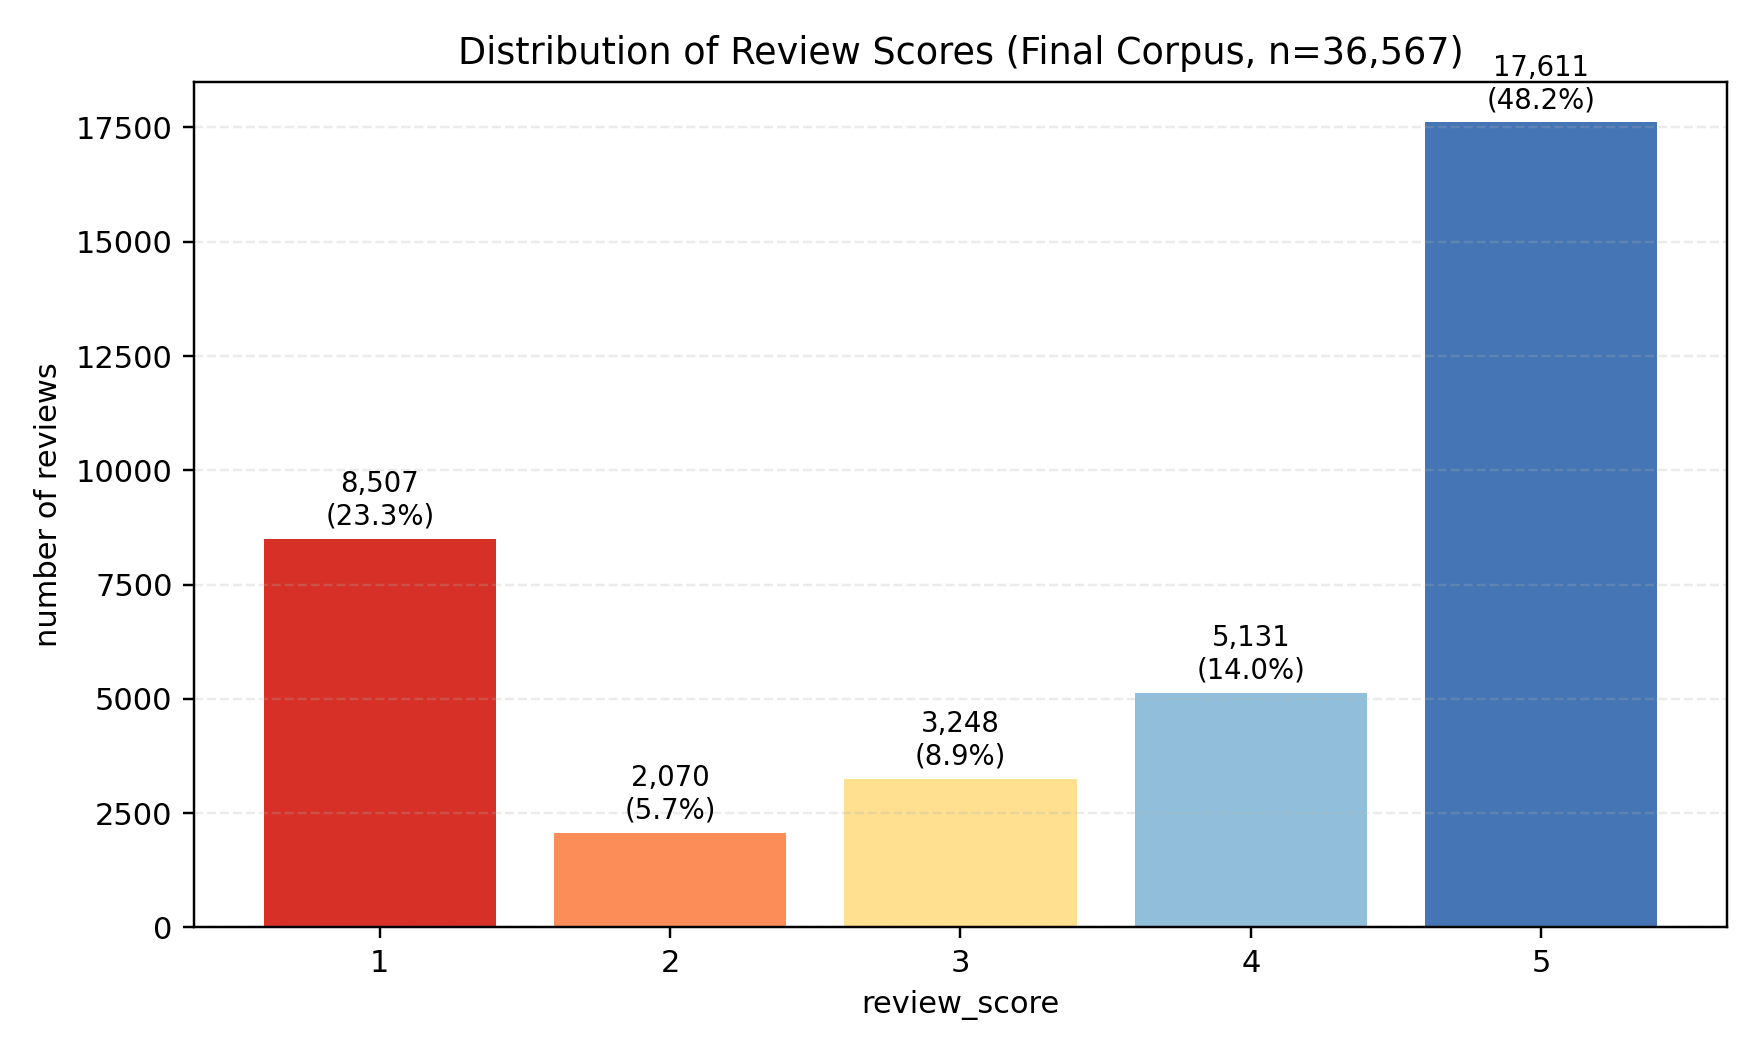
\includegraphics[width=\linewidth]{olist_negative_sentiment_geometry_assets/figures/phase1_rating_distribution.png}
\caption{\textit{Review score distribution in the final corpus (n = 36{,}567).}}
\label{fig:phase1-rating-distribution}
\end{figure}

\subsection{Text Preprocessing}
\label{subsec:preproc}

Text preprocessing aims to standardise the review messages while preserving information relevant for semantic modelling. 
Starting from the raw comments, I apply the following steps:

\begin{enumerate}
    \item Lowercasing all text.
    \item Removing URLs, HTML tags, digits, and most punctuation via regular expressions.
    \item Normalising whitespace and stripping leading/trailing spaces.
    \item Dropping reviews whose cleaned text falls below a minimum length threshold.
\end{enumerate}

To choose the length threshold, I evaluate how many reviews would be retained at different minimum numbers of characters. 
A threshold of 12 characters keeps about 90\% of the non-empty baseline while discarding extremely short or non-informative messages (for example, single-word reactions such as ``bom'' or ``ok''). 
This trade-off results in the final set of 36{,}567 reviews mentioned above.

I also considered more aggressive normalisation such as stemming. 
On this corpus, stemming would almost halve the vocabulary size without shortening reviews, and would merge many distinct Portuguese surface forms onto the same stems, making qualitative examples less readable. 
For this project, I therefore keep a non-stemmed, stopword-filtered version of the cleaned text, denoted \texttt{clean\_text}, which is used as input to all embedding models.

\subsection{Primary Sentiment Labels}
\label{subsec:rating-group}
The dataset provides a 1--5 star rating for each review. 
For the purposes of geometric analysis, I collapse these scores into a coarse three-level sentiment variable \texttt{rating\_group}:
\begin{itemize}
    \item 1--2 stars: \emph{negative}
    \item 3 stars: \emph{neutral}
    \item 4--5 stars: \emph{positive}
\end{itemize}
This mapping follows common practice in review mining and balances class sizes while preserving a clear negative versus positive contrast.

In the final corpus, negative reviews (1--2 stars) form approximately 29\% of all examples, neutral reviews (3 stars) about 9\%, and positive reviews (4--5 stars) about 62\%. 
Combined with the length differences noted above, this indicates that the corpus contains sufficiently many and sufficiently rich negative examples to support the analysis of geometric structure.

In this study, I deliberately use the three-way star label as the \emph{primary} sentiment signal (\texttt{rating\_group}). 
Star ratings represent the user's own explicit judgement at the time of review and are the labels that business systems typically try to predict or explain. 
Lexicon-based methods, in contrast, operate on surface word polarity and may underestimate dissatisfaction expressed through polite or indirect language. 
Since the goal of this work is to understand how embedding spaces organise reviews with respect to the labels actually observed by the platform, \texttt{rating\_group} is used in all cluster-purity, homophily, and islandisation metrics, while lexicon-based signals play a supporting, diagnostic role.

\subsection{Lexicon-based Sentiment Probe}
Star ratings capture the overall user judgement but do not directly reflect the polarity of the words used in the text. 
As an independent textual sentiment probe, I therefore use the Portuguese OpLexicon v3.0 lexicon, a manually curated resource with roughly 32k entries annotated with polarity scores. 
For each review, I tokenise \texttt{clean\_text}, sum the polarities of words present in the lexicon, and obtain a real-valued score \texttt{lexicon\_score}. 
Based on the sign of this score, I derive a categorical variable \texttt{lexicon\_group} with values \emph{negative}, \emph{neutral}, and \emph{positive}.

I use OpLexicon v3.0 rather than training a separate supervised classifier or adopting a multilingual lexicon for two reasons. 
First, OpLexicon is specifically designed for Portuguese and covers many domain-relevant polarity terms, which makes it suitable as a lightweight, language-appropriate probe without additional training. 
Second, using a fixed lexicon avoids re-introducing model-specific biases at this stage: the goal is to contrast user ratings with a simple, transparent textual polarity signal, not to build another complex sentiment model whose behaviour would itself require interpretation.

Cross-tabulating rating groups and lexicon groups shows only moderate agreement (around 46\% overall). 
Positive ratings align best with lexical polarity: the majority of 4--5-star reviews are lexically positive and only a small fraction are lexically negative. 
In contrast, negative ratings are dominated by ``polite negatives'': only about a quarter of 1--2-star reviews are lexically negative, while the remainder use neutral or even positive words. 
There is also a smaller set of ``mixed positives'', where 4--5-star reviews contain clearly negative terms despite the high rating. 
These patterns confirm that star ratings compress nuanced textual sentiment, especially for negative and neutral classes. 
In the analysis, \texttt{rating\_group} remains the primary sentiment label used for geometric probing, while \texttt{lexicon\_group} is used only as an auxiliary probe to interpret mismatches between ratings and text and to motivate why geometry should not rely solely on surface polarity words.

\begin{table}[tbp]
\centering
\small
\caption{\textit{Rating vs Lexicon Agreement Metrics}}
\label{tab:data-lexicon-agreement}
\begin{tabular}{lc}
\toprule
\textbf{Metric} & \textbf{Value} \\
\midrule
Overall agreement & 45.89\% \\
Polite negative rate & 21.55\% \\
Mixed positive rate & 3.88\% \\
Number of reviews & 36{,}567 \\
\bottomrule
\end{tabular}
\end{table}

\begin{figure}[tbp]
\centering
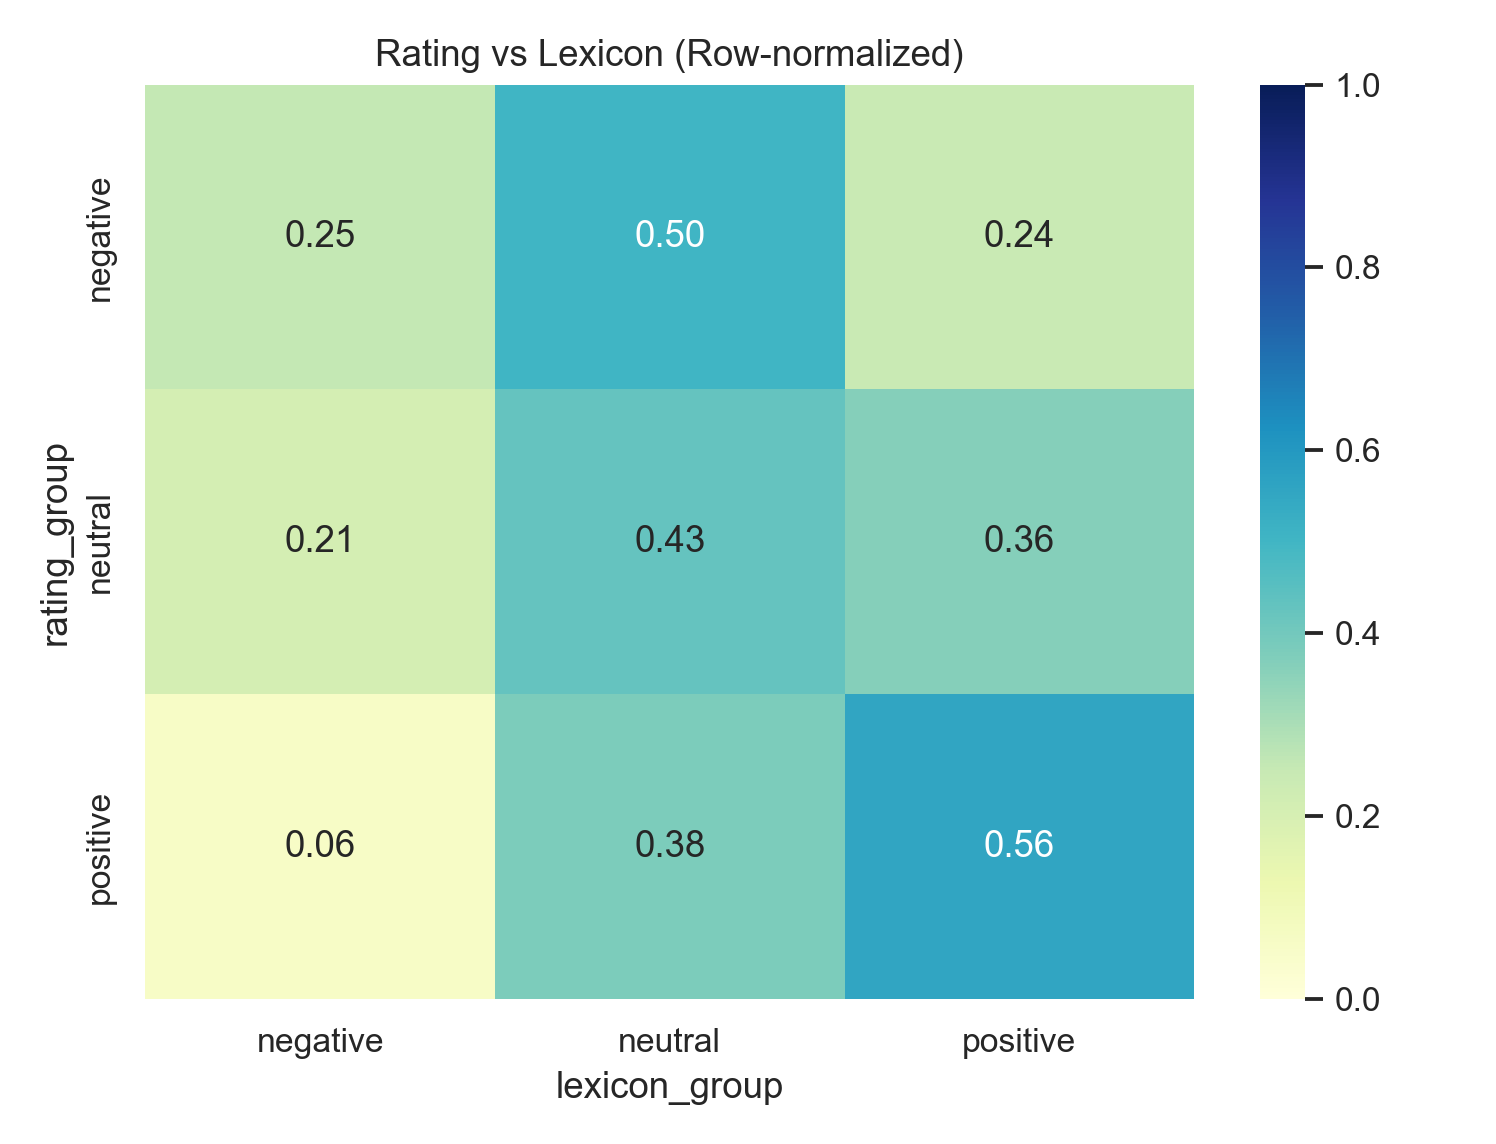
\includegraphics[width=\linewidth]{olist_negative_sentiment_geometry_assets/figures/phase1_rating_vs_lexicon_rownorm_heatmap.png}
\caption{\textit{Row-normalised cross-tabulation between rating-based sentiment and lexicon-based sentiment.}}
\label{fig:data-rating-lexicon-heatmap}
\end{figure}

\subsection{Regex-based Topic Proxy}

To obtain a simple notion of topic that is independent of any embedding model, I construct a regex-based topic proxy over \texttt{clean\_text}. 
A small set of manually designed keyword patterns assigns each review to one of the following broad categories:

\begin{itemize}
    \item \textbf{delivery}: shipping time, non-delivery, delays (e.g., ``entrega'', ``chegou'', ``prazo'', ``no recebi'');
    \item \textbf{product}: product quality, defects, descriptions (e.g., ``produto'', ``qualidade'', ``defeito'', ``veio quebrado'');
    \item \textbf{support}: customer service and communication (e.g., ``atendimento'', ``suporte'', ``vendedor'');
    \item \textbf{refund}: returns, reimbursements, cancellations (e.g., ``troca'', ``reembolso'', ``devolu\c{c}\~ao'', ``cancelamento'');
    \item \textbf{price}: cost, promotions, value for money (e.g., ``pre\c{c}o'', ``promo\c{c}\~ao'', ``barato'', ``caro'');
    \item \textbf{other}: reviews that do not match any of the above patterns.
\end{itemize}

This proxy is intentionally coarse and noisy. 
Many reviews mention multiple aspects, and some fall into the \emph{other} bucket because they use more indirect language or refer to issues not covered by the patterns. 
In the final corpus, \textbf{delivery} and \textbf{product} dominate the proxy distribution (about 37.11\% and 30.30\%), while \textbf{other} still captures a substantial share (28.98\%). 
The remaining categories (\textbf{support}, \textbf{refund}, \textbf{price}) are comparatively small but still useful as weak service-dimension signals. 

\begin{table}[tbp]
\centering
\small
\caption{\textit{Regex Topic Proxy Distribution on the Final Corpus}}
\label{tab:data-topic-proxy-distribution}
\adjustbox{max width=\linewidth}{
\begin{tabular}{lcc}
\toprule
\textbf{Topic proxy} & \textbf{Reviews} & \textbf{Share (\%)} \\
\midrule
delivery & 13{,}570 & 37.11 \\
product & 11{,}078 & 30.30 \\
support & 678 & 1.85 \\
refund & 351 & 0.96 \\
price & 294 & 0.80 \\
other & 10{,}596 & 28.98 \\
\bottomrule
\end{tabular}
}
\end{table}

\begin{figure}[tbp]
\centering
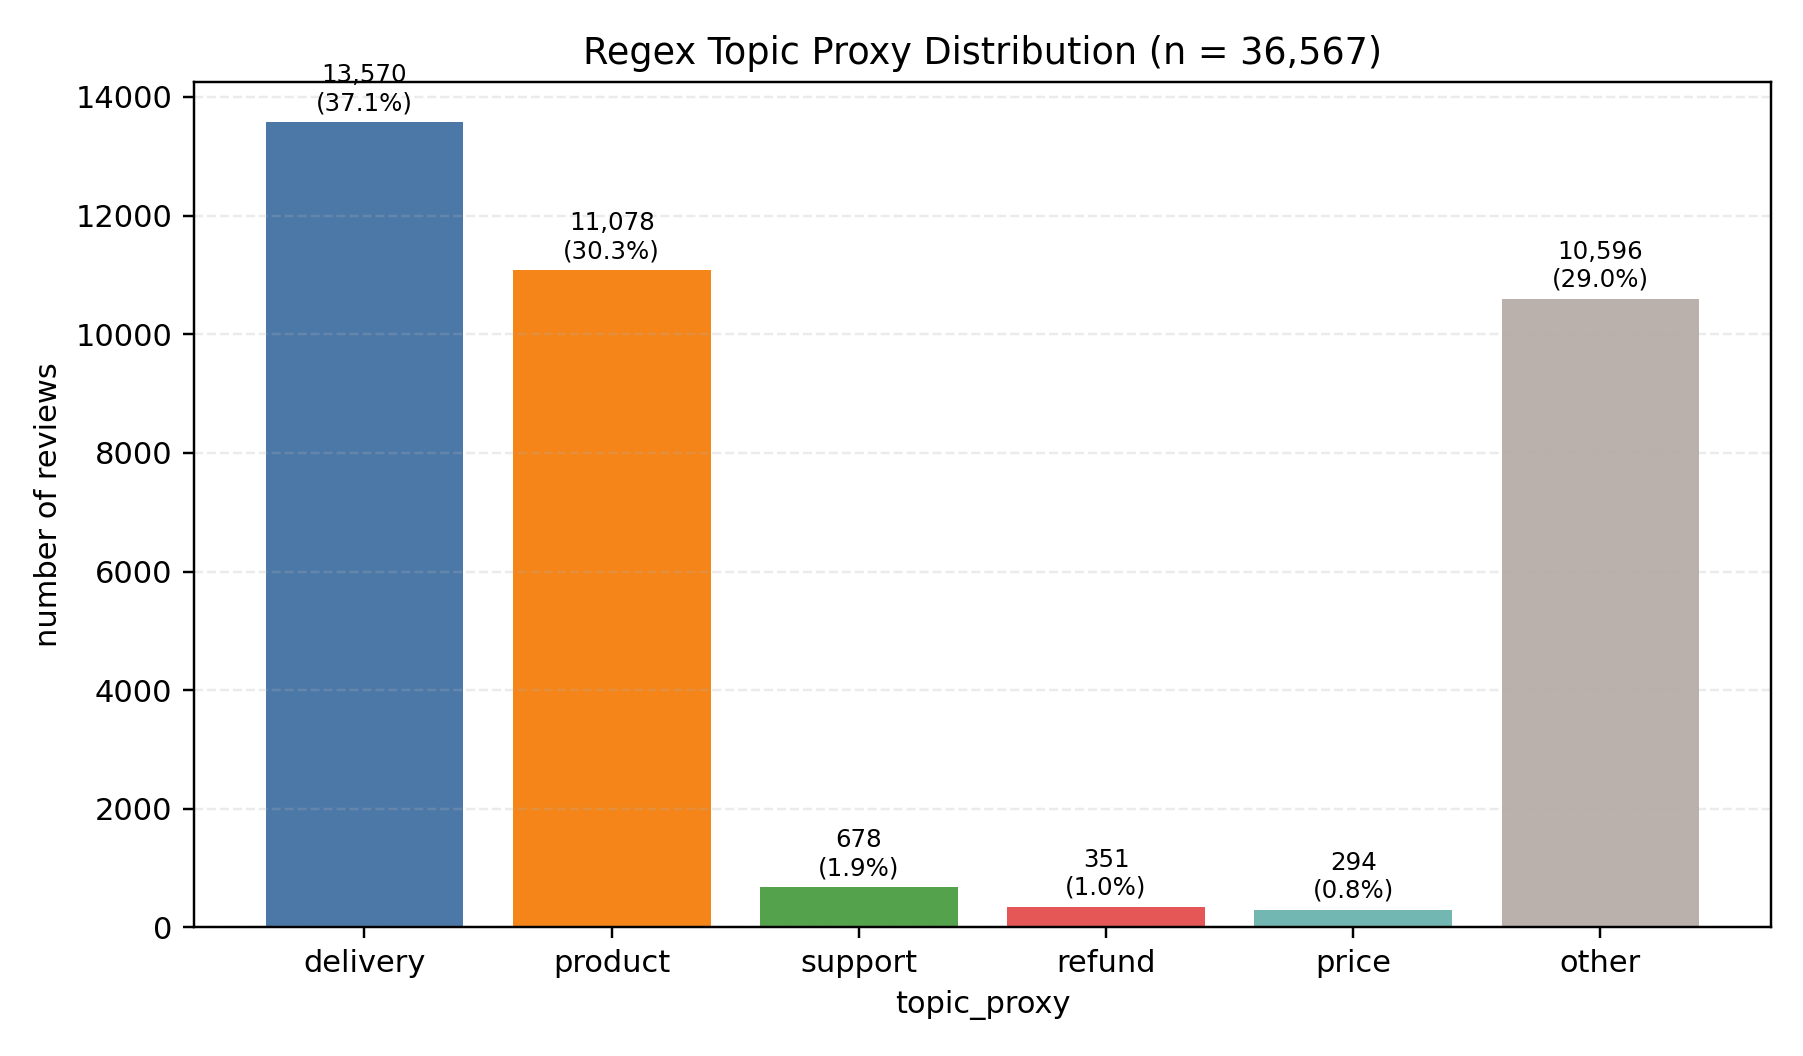
\includegraphics[width=\linewidth]{olist_negative_sentiment_geometry_assets/figures/phase1_topic_proxy_distribution.png}
\caption{\textit{Distribution of regex-based topic proxy labels (n = 36{,}567).}}
\label{fig:data-topic-proxy-distribution}
\end{figure}

The goal of this labelling is not to provide a perfect topic annotation, but to create a simple, model-independent reference against which I can measure how much the embedding-based clusters align with topical versus sentiment structure in the geometric analysis that follows.
\section{Methods}
\label{sec:methods}

The goal of this study is to compare how different embedding models organise Brazilian e-commerce reviews with respect to sentiment and coarse topics. 
Methodologically, I treat each embedding space as a geometric object and ask where negative reviews are located, how concentrated they are, and how this behaviour changes across models. 
This section describes the embedding extraction process, the clustering and projection procedures used to expose global structure, and the geometry-aware metrics that quantify negative ``islands'' versus diffuse layers in a way that is comparable across models.

For qualitative inspection in tables and figures, I link Portuguese reviews to the external English translation companion dataset from Kaggle \citep{olist_reviews_translated_kaggle} using \texttt{review\_id}. 
These English snippets are used only for interpretation in the paper and do not enter embedding extraction or any quantitative analysis.

\subsection{Embedding Models and Dense Vectors}
\label{subsec:embeddings}

I encode each review into a dense vector representation by applying three pre-trained embedding models to \texttt{clean\_text}. 
Each model maps the input sentence to a point in a high-dimensional continuous space, so that semantically similar reviews are expected to lie close to each other in terms of cosine distance.

The three models are:

\begin{itemize}
    \item \textbf{BERTimbau}: a monolingual transformer encoder pre-trained on large Brazilian Portuguese corpora \citep{bertimbau-paper}. It is expected to capture fine-grained Portuguese morphology and idiomatic usage, which should be beneficial for the Olist reviews.
    \item \textbf{Multilingual MiniLM}: a compact sentence-transformer trained on multiple languages \citep{minilm-paper,reimers-gurevych-sbert}. It provides efficient sentence-level embeddings optimised for semantic similarity, but may trade language-specific nuances for cross-lingual robustness.
    \item \textbf{OpenCLIP text encoder}: the text tower of a vision--language contrastive model \citep{clip-paper,openclip-paper}. Its semantic space is shaped by cross-modal alignment rather than purely textual objectives, offering a qualitatively different representation of review content.
\end{itemize}

For each model, I obtain a single fixed-dimensional vector per review from the recommended sentence representation (for example, pooled \texttt{[CLS]} token or mean-pooled token embeddings). 
The resulting dimensions are 768 for BERTimbau, 384 for Multilingual MiniLM, and 512 for the OpenCLIP text encoder. 
To make cosine similarity comparable across models and to stabilise downstream methods, I apply $\ell_2$ normalisation to every vector: for an embedding $x \in \mathbf{R}^d$, I use $\tilde{x} = x / \|x\|_2$. 
In this representation, cosine similarity between two reviews reduces to the dot product $\tilde{x}_i^\top \tilde{x}_j$, and all vectors lie on the unit hypersphere, which is a common assumption in geometric analyses of embeddings.

To analyse local structure, I also treat each embedding space as an implicit $k$-nearest neighbour graph: 
for every review, I can retrieve its $k$ closest neighbours in the dense vector space using cosine distance. 
This graph underlies both the qualitative neighbour inspections and the quantitative homophily metrics described later in Section~\ref{subsec:island-metrics}. 
As an initial qualitative check, I inspect $k$-nearest neighbours for a small set of anchor reviews (for example, non-delivery complaints and highly positive delivery praise) in each embedding space; neighbours are semantically coherent in all models, but differ in how sentiment-homogeneous they are, which motivates the more systematic analysis below.

\subsection{Geometry and Clustering}
\label{subsec:geometry-clustering}

To expose global structure in each embedding space, I use unsupervised clustering and examine how the resulting partitions align with sentiment and topic labels. 
This follows the use of purity and silhouette-based diagnostics in prior work on representation learning, adapted here to the specific question of sentiment versus topic organisation \citep{manning-ir-book}.

\paragraph{K-Means diagnostics and fixed-$k$ protocol.}

For each embedding model, I first explore K-Means clustering on $\ell_2$-normalised embeddings using a stratified diagnostic sample of 4{,}000 reviews, and evaluate partitions with cosine-based internal metrics. 
I vary the number of clusters $k \in \{2,4,6,7,8,10,12\}$ and, for each value of $k$, compute several standard internal validation metrics:

\begin{itemize}
    \item cosine silhouette score, which measures how much closer points are to their own cluster than to neighbouring clusters;
    \item Calinski--Harabasz index, which favours compact, well-separated clusters;
    \item Davies--Bouldin index, which penalises overlapping clusters;
    \item within-cluster inertia, i.e. the sum of squared distances to cluster centroids.
\end{itemize}
These are standard internal clustering diagnostics \citep{rousseeuw-silhouette,calinski-harabasz,davies-bouldin}.

I use these diagnostics as a structure check and then apply a fixed cross-model partition size, $k=7$, to preserve comparability and maintain interpretable topic granularity across embedding families.
I repeat clustering with several random initialisations and find that cluster sizes remain well balanced (roughly 10--21\% of reviews per cluster) and internal metrics vary only marginally, indicating stable partitions.

\paragraph{Cluster purity for sentiment and topic.}

Given the K-Means assignments, I quantify how strongly clusters align with sentiment and topic labels using cluster purity, a standard measure in clustering evaluation. 
For a generic label $y$ (either the primary sentiment \texttt{rating\_group} or the regex-based topic proxy), cluster purity is defined as
\[
\text{purity}(y) = \frac{1}{N} \sum_{c} \max_{\ell} \left| \{ i : \hat{c}(i) = c,\; y_i = \ell \} \right|,
\]
where $N$ is the number of reviews, $\hat{c}(i)$ is the cluster assignment of review $i$, and $\ell$ ranges over the possible label values. 
Intuitively, purity measures the fraction of reviews that belong to the majority label in their cluster.

As a simple illustration, suppose there are $N = 1{,}000$ reviews and three clusters. 
If cluster 1 contains 300 reviews of which 240 are negative, cluster 2 contains 400 reviews of which 260 are positive, and cluster 3 contains 300 reviews of which 210 are positive, then the majority label counts are $(240, 260, 210)$ and the purity is
\[
\text{purity} = \frac{240 + 260 + 210}{1{,}000} = 0.71.
\]
If, for the same clustering, the topic proxy labels are much more mixed inside each cluster, the corresponding purity for topic will be lower, indicating that the clusters are more sentiment-oriented than topic-oriented.

In the experiments, I compute purity for both sentiment and topic in each embedding model using the fixed-$k$ K-Means partition.
This K-Means solution serves as the reference for the more detailed islandisation metrics described in Section~\ref{subsec:island-metrics}.

\subsection{Projection and Visual Diagnostics}
\label{subsec:projection-visual}

Clustering summarises global structure but does not by itself reveal how clusters and labels are arranged in space. 
To obtain interpretable views of the geometry, I project embeddings into two dimensions and use standard visual diagnostics, without drawing conclusions in this section.

\paragraph{PCA, t-SNE, and UMAP projections.}

I use three complementary projection methods \citep{jolliffe-pca,maaten-hinton-tsne,mcinnes-umap}:

\begin{itemize}
    \item \textbf{PCA}: a linear projection that finds orthogonal directions of maximum variance. I fit PCA on all embeddings for a given model and use the first two principal components.
    \item \textbf{t-SNE}: a non-linear method that approximately preserves local neighbourhood structure. I use cached full-dataset t-SNE coordinates when available; if a cache is missing, I compute a fallback map on a stratified subsample (up to about 3{,}000 points), using perplexity 35 and up to 1{,}200 iterations.
    \item \textbf{UMAP}: a manifold-learning technique that seeks to preserve both local and some global structure. As with t-SNE, I use cached full-dataset UMAP coordinates when available, and otherwise compute a sampled fallback with 20 neighbours and minimum distance 0.05.
\end{itemize}

For each model and projection method, I prepare scatter plots coloured by K-Means cluster ID and by sentiment label \texttt{rating\_group}. 
I also prepare a topic-overlay diagnostic where sentiment-coloured points are combined with translucent topic-region circles derived from the regex topic proxy, so topical concentration can be inspected without replacing sentiment encoding.
These plots, presented later in the Results section, provide an intuitive sense of whether clusters correspond to well-separated regions and whether negative reviews tend to occupy specific lobes or appear as a layer spread across the map.

\paragraph{2D silhouette comparison for sentiment and topic.}

To complement visual inspection with a simple quantitative diagnostic, I compute silhouette scores on the 2D projections for both sentiment and topic labels. 
Given projected coordinates $z_i \in \mathbf{R}^2$ and a label $y$, the silhouette score of point $i$ is
\[
s_i = \frac{b_i - a_i}{\max(a_i, b_i)},
\]
where $a_i$ is the average distance from $i$ to points with the same label and $b_i$ is the smallest average distance from $i$ to points with a different label. 
The overall silhouette is the mean of $s_i$ across all points.

For example, if reviews with the same sentiment lie close together in the projection while reviews with different sentiments are far apart, the silhouette for sentiment might approach $0.4$ or $0.5$, whereas if sentiment labels are intermixed the silhouette will be near $0$. 
By computing silhouettes with respect to \texttt{rating\_group} and the topic proxy on the same 2D coordinates, I can see whether the low-dimensional maps preserve sentiment structure more strongly than topic structure and how this pattern varies across embedding models.

\paragraph{$k$-nearest neighbour neighbourhood plots.}

Finally, I use $k$-nearest neighbour diagnostics as a local visual tool. 
For selected anchor reviews (for example, prototypical negative and positive cases within specific topics), I highlight their positions and those of their $k$ nearest neighbours in the 2D projections, colouring points by sentiment or topic. 
This visualises the same idea as the homophily metric introduced below: if neighbours of a negative anchor are mostly negative, this suggests local island-like structure; if they are mixed, it suggests a more diffuse arrangement. 
These neighbourhood plots are not used for formal evaluation but help interpret the quantitative results.

\subsection{Islandisation Metrics}
\label{subsec:island-metrics}

The central methodological contribution of this paper is a small set of metrics that capture how ``island-like'' negative reviews are in each embedding space. 
Their design is inspired by previous work on homophily and dispersion in graph-based analyses, but adapted to high-dimensional review embeddings \citep{newman-mixing}.

\paragraph{Cluster-wise negative ratios and dispersion.}

Given the K-Means clustering with $k = 7$ and the primary sentiment label \texttt{rating\_group}, I compute, for each cluster $c$,
\[
r_c = \frac{\text{\# negative reviews in } c}{\text{\# all reviews in } c}.
\]
I also compute the global negative rate
\[
\bar{r} = \frac{\text{\# all negative reviews}}{N}
\]
and the standard deviation of the cluster-wise negative ratios,
\[
\sigma_r = \sqrt{\frac{1}{k} \sum_{c} (r_c - \bar{r})^2}.
\]

A small $\sigma_r$ indicates that negative reviews are distributed fairly evenly across clusters (diffuse pattern), whereas a large $\sigma_r$ means that some clusters are much more negative than others (island-like pattern). 
For example, if the global negative rate is $\bar{r} = 0.29$ and the cluster-wise ratios are $(0.31, 0.27, 0.30, 0.28, 0.29, 0.30, 0.27)$, then $\sigma_r$ is close to zero and no cluster deviates strongly from the average. 
In contrast, if some clusters have $r_c$ near $0.10$ and others near $0.70$, $\sigma_r$ becomes much larger, signalling that negatives concentrate in a few clusters. 
In practice I inspect $r_c - \bar{r}$ and simple binomial confidence intervals per cluster to identify clusters that are significantly more or less negative than the corpus average.
A high $\sigma_r$ alone does not uniquely identify one geometric pattern: it can arise either from one or two very negative clusters (peaky islandisation) or from several moderately negative clusters (diffuse concentration). 
For this reason, I report both $\sigma_r$ and the explicit island flag based on joint negative-ratio and density thresholds; the qualitative RQ1 label is \textit{islands} when at least one cluster is flagged, and \textit{diffuse} otherwise.

\paragraph{Negative homophily in $k$-nearest neighbour graphs.}

To capture local structure independently of K-Means, I build a $k$-nearest neighbour graph in each embedding space, using $k = 20$ and cosine distance (illustrative local map in Figure~\ref{fig:knn-neighbourhoods}). 
For every negative review $i$, I compute the fraction of its neighbours that are also negative:
\[
h_i = \frac{1}{k} \sum_{j \in \mathcal{N}_k(i)} \mathbf{1}\{ y_j = \text{negative} \},
\]
where $\mathcal{N}_k(i)$ is the set of $k$ nearest neighbours of $i$ and $y_j$ is the sentiment label of review $j$. 
The overall negative homophily is the average of $h_i$ over all negative reviews. 

If negative sentiment forms islands, homophily should be noticeably higher than the global negative rate $\bar{r}$. 
For instance, if $\bar{r} = 0.29$ but a typical negative review has around 14 negative neighbours out of 20 ($h_i \approx 0.70$), then negative reviews are much more likely to be close to other negatives than random chance would suggest. 
If, on the other hand, homophily stays close to $\bar{r}$ (for example, $h_i \approx 0.32$), this indicates a more diffuse configuration.

\paragraph{Within-class dispersion.}

To assess how tight or spread out different label groups are, I measure within-class dispersion using pairwise cosine distances. 
For a label group $G$ (for example, negative reviews or a given topic category), let $D_G$ denote the average pairwise distance between all pairs of reviews in $G$. 
I compute $D_G$ for each sentiment group and for each topic proxy category and normalise by the overall average pairwise distance on the corpus. 

For example, if the global average pairwise distance is $0.50$ and the average distance among negative reviews is $0.42$, the normalised dispersion for negatives is $0.84$, indicating that negative reviews tend to form tighter regions than the corpus as a whole. 
If positive reviews instead have a normalised dispersion close to $1.0$, they are as spread out as the average review, suggesting that tight structure is more characteristic of negative content.

\paragraph{Negative islands and their mass.}

Combining cluster-wise negative ratios and an approximate measure of cluster density (for example, inverse average pairwise distance within each cluster), I define \emph{negative islands} as clusters that satisfy both:
\begin{itemize}
    \item $r_c$ is higher than the global negative rate $\bar{r}$ by at least one standard deviation; and
    \item the cluster has above-average density compared to other clusters in the same model.
\end{itemize}

For each embedding model, I record (i) the number of such negative islands and (ii) the \emph{negative island mass}, defined as the share of all reviews that belong to island-flagged clusters. 
As an illustration, if island clusters contain 20\% of all reviews, the island mass is 0.20; if no cluster satisfies the criteria, island mass is 0.

\paragraph{Bootstrap comparison across models.}

To compare islandisation strength across models in a way that reflects sampling uncertainty, I use bootstrap resampling at the cluster level. 
This follows standard non-parametric bootstrap practice \citep{efron-tibshirani-boot}.
For each embedding model, I repeatedly resample the seven clusters with replacement, recompute $\sigma_r$ and negative island mass on each resample, and obtain empirical confidence intervals for these metrics. 
I then estimate the distribution of differences between models (for example, $\sigma_r^{\text{BERTimbau}} - \sigma_r^{\text{MiniLM}}$) to see whether one model consistently exhibits stronger or weaker islandisation than another.

For example, if the bootstrap distribution of $\sigma_r^{\text{BERTimbau}} - \sigma_r^{\text{MiniLM}}$ is mostly positive and its 95\% confidence interval does not cross zero, this suggests that BERTimbau produces more uneven negative ratios across clusters than MiniLM and therefore stronger island-like structure. 
This non-parametric bootstrap follows the general idea of comparing representation spaces via resampled summary statistics rather than relying on single-point estimates. 
Together with the homophily and dispersion measures, it provides a quantitative basis for answering RQ1 (islands versus diffuse layer) and RQ2 (differences in islandisation strength across BERTimbau, Multilingual MiniLM, and OpenCLIP).

\section{Experimental Results}
\label{sec:results}

This section reports the empirical findings of the analysis. 
I first summarise basic embedding behaviour and cluster structure, then examine how clusters align with sentiment and topics, and finally present the islandisation metrics that directly address RQ1 and RQ2.

\subsection{Embedding Behaviour and Neighbourhoods}

Before analysing geometry, I inspect the basic properties of the three embedding spaces. 
Prior to normalisation, the models produce vectors with very different norms: BERTimbau embeddings have an average $\ell_2$ norm of about $7.8$, Multilingual MiniLM about $3.3$, and OpenCLIP about $10.4$, each with substantial spread. 
After $\ell_2$ normalisation, all models have norms essentially equal to 1 with near-zero variance, confirming that the preprocessing step successfully standardises vector length and makes cosine similarity directly comparable within and across models.

Table~\ref{tab:embedding-norms-results} reports these norm diagnostics and the embedding dimensionality used in subsequent phases.

\begin{table}[tbp]
\centering
\small
\caption{Embedding norm diagnostics after extraction and $\ell_2$ normalisation.}
\label{tab:embedding-norms-results}
\adjustbox{max width=\linewidth}{
\begin{tabular}{lccc}
\hline
\textbf{Model} & \textbf{Dim} & \textbf{Raw norm ($\mu \pm \sigma$)} & \textbf{$\ell_2$ norm mean} \\
\hline
BERTimbau & 768 & $7.68 \pm 0.64$ & $1.00$ \\
MiniLM    & 384 & $3.24 \pm 0.46$ & $1.00$ \\
OpenCLIP  & 512 & $10.48 \pm 1.02$ & $1.00$ \\
\hline
\end{tabular}
}
\end{table}

The $k$-nearest neighbour sanity checks show that all models retrieve semantically coherent neighbours around anchor reviews. 
For clearly positive delivery-praise anchors (for example, ``chegou antes do prazo, bem embalado''), the closest neighbours in all three spaces describe early or on-time delivery and good packaging, and virtually all share the positive sentiment label. 
For more ambiguous anchors (for example, delivery on time but refused or cancelled orders), BERTimbau’s neighbours tend to be more sentiment-homogeneous than those of MiniLM and OpenCLIP, which already hints at different ways in which the three spaces encode local sentiment structure.

\subsection{Cluster Structure and Stability}

Using the common protocol described in Section~\ref{sec:methods}, I apply K-Means clustering on $\ell_2$-normalised embeddings and evaluate cluster quality with cosine-based diagnostics in each embedding space. 
On the stratified diagnostic sample (4{,}000 rows per model), the highest raw silhouette appears at low $k$ (especially $k=2$), while the 6--8 range yields finer partitions with comparable internal quality. 
For cross-model comparability and interpretable topic granularity, I fix a common $k = 7$ and use this partition for all downstream analyses.
Additional checks at $k \in \{6,8\}$ show similar qualitative patterns for purity and islandisation, suggesting that the main conclusions are not an artefact of choosing $k=7$.

Figure~\ref{fig:phase3-kcurve-silhouette} shows the K-curve trend used to justify this common choice.

\begin{figure}[tbp]
\centering
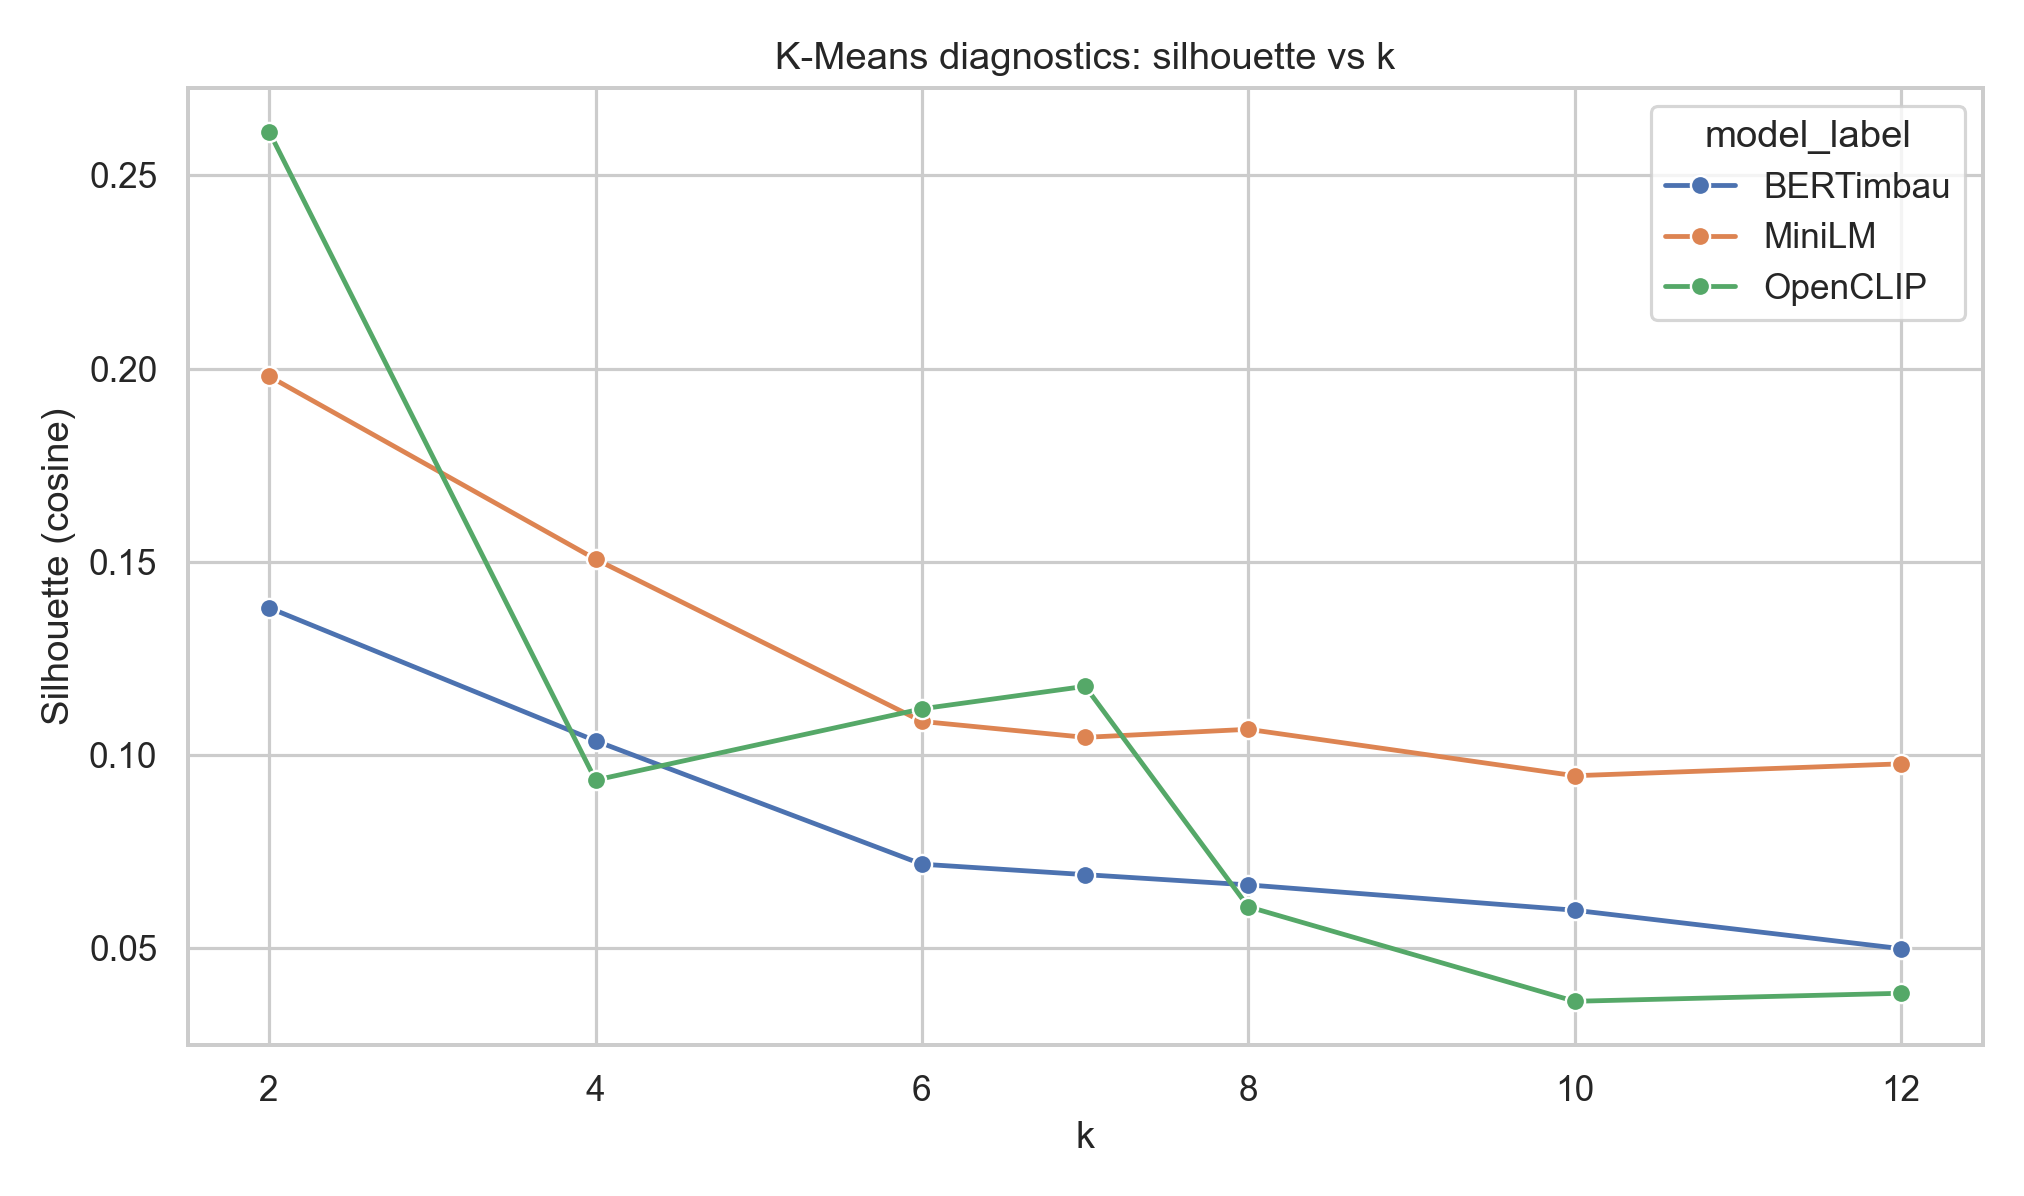
\includegraphics[width=\linewidth]{olist_negative_sentiment_geometry_assets/figures/phase3_kmeans_kcurve_silhouette.png}
\caption{K-Means silhouette diagnostics across $k$ on the stratified diagnostic sample ($n=4{,}000$ per model).}
\label{fig:phase3-kcurve-silhouette}
\end{figure}

Table~\ref{tab:cluster-quality} summarises the resulting cluster quality.

\begin{table}[tbp]
\centering
\small
\adjustbox{max width=\linewidth}{
\begin{tabular}{lcc}
\hline
\textbf{Model} & \textbf{K-Means $k$} & \textbf{Silhouette} \\
\hline
BERTimbau           & 7 & 0.07 \\
Multilingual MiniLM & 7 & 0.10 \\
OpenCLIP text       & 7 & 0.06 \\
\hline
\end{tabular}
}
\caption{Cluster quality per embedding model (fixed $k=7$).}
\label{tab:cluster-quality}
\end{table}

Under the fixed-$k$ protocol, all three embedding spaces are partitioned into seven substantial clusters: cluster sizes range from about 10\% to 21\% of the corpus, with no tiny or degenerate groups.
Stability checks across multiple K-Means seeds show very small variation in silhouette and inertia, indicating that the seven-cluster geometry is not an artefact of initialisation.

\begin{figure}[tbp]
\centering
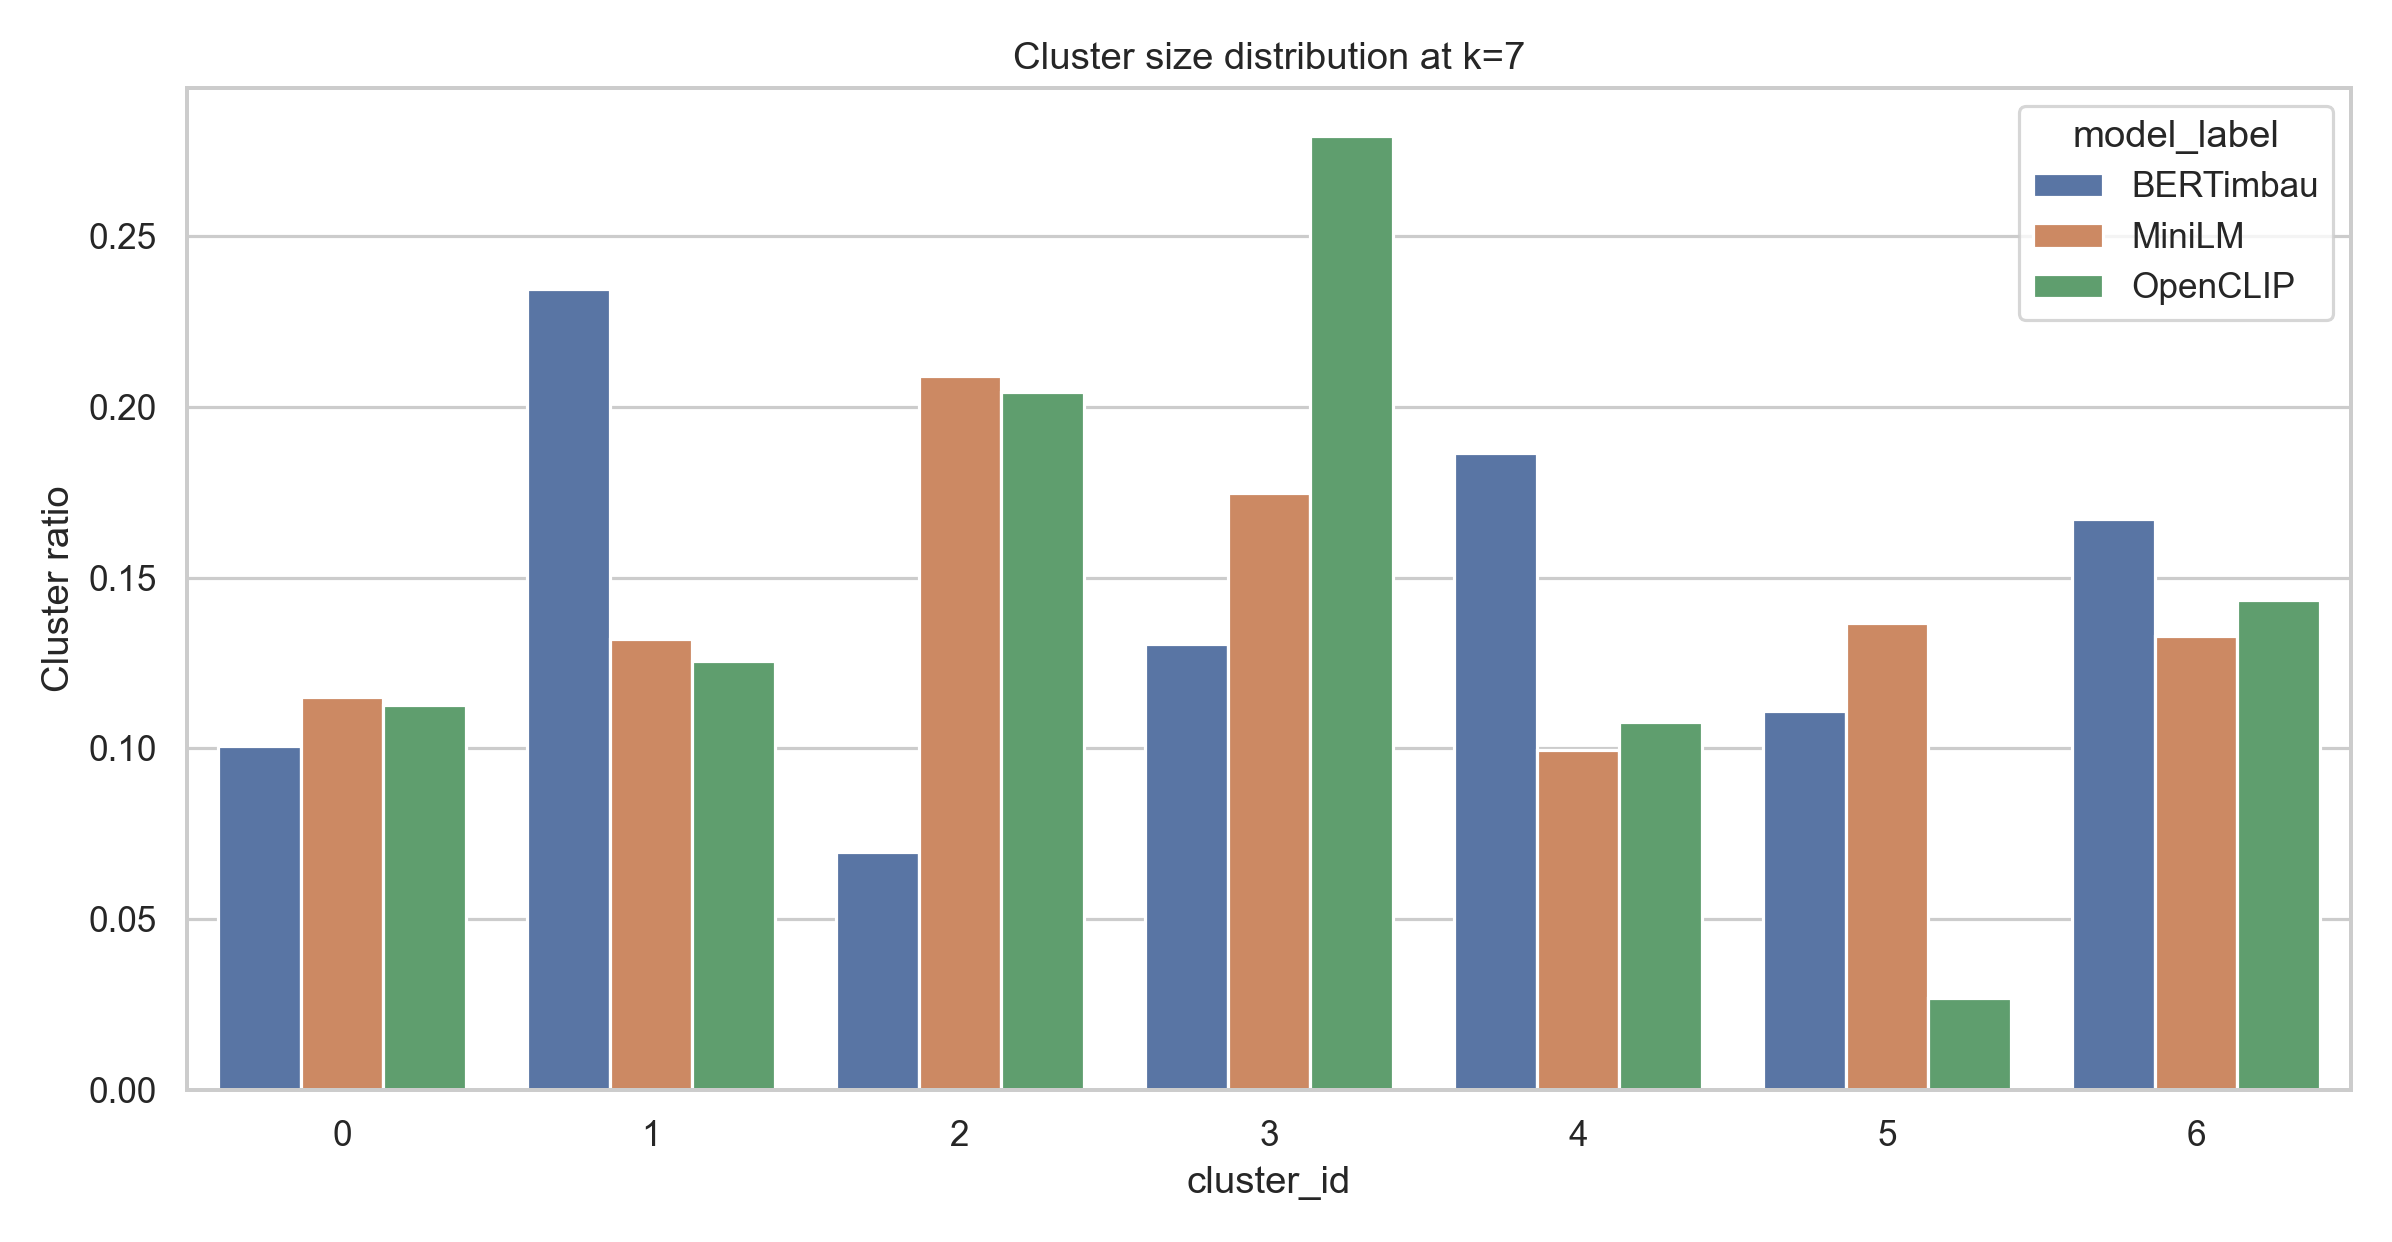
\includegraphics[width=\linewidth]{olist_negative_sentiment_geometry_assets/figures/phase3_cluster_size_distribution_k7.png}
\caption{Cluster size distribution at $k=7$ across BERTimbau, MiniLM, and OpenCLIP.}
\label{fig:phase3-cluster-size-dist}
\end{figure}

\subsection{Sentiment and Topic Purity}

To assess whether clusters are primarily organised by sentiment or by the regex-based topic proxy, I compute cluster purity for both label sets. 
Table~\ref{tab:purity} reports purity values for the fixed-$k$ K-Means solution.

\begin{table}[tbp]
\centering
\small
\adjustbox{max width=\linewidth}{
\begin{tabular}{lccc}
\hline
\textbf{Model} & \textbf{Purity (sent.)} & \textbf{Purity (topic)} & \textbf{$\Delta$ (sent-topic)} \\
\hline
BERTimbau           & 0.756 & 0.595 & 0.161 \\
Multilingual MiniLM & 0.792 & 0.563 & 0.229 \\
OpenCLIP text       & 0.668 & 0.513 & 0.155 \\
\hline
\end{tabular}
}
\caption{Cluster purity with respect to sentiment and regex-based topic proxy (fixed $k=7$ K-Means).}
\label{tab:purity}
\end{table}

Across all models, sentiment purity is higher than topic purity, with gaps between 0.155 and 0.229 points.
Multilingual MiniLM has the highest sentiment purity (0.792), BERTimbau is slightly lower (0.756), and OpenCLIP has the lowest (0.668), while topic purity is moderate (0.513--0.595).
This indicates that, given the coarse topic proxy, emergent clusters are more sentiment-oriented than topic-oriented, and that MiniLM’s geometry separates sentiment labels most cleanly.

\subsection{Projections and 2D Diagnostics}

PCA, t-SNE, and UMAP projections provide a visual ``semantic map'' of each embedding space. 
In all three models, projections reveal a single large cloud of reviews rather than many disconnected blobs, within which the selected seven clusters form visible patches, especially in PCA and t-SNE for BERTimbau and MiniLM. 
OpenCLIP’s clusters overlap more strongly and appear more elongated, reflecting its lower sentiment purity.

For readability, I present cluster-coloured and sentiment-coloured maps as separate figures rather than a single dual-encoding overlay. 
When colouring the same projections by \texttt{rating\_group}, positive, neutral, and negative reviews form overlapping layers rather than perfectly separated islands. 
However, some regions are visibly more negative than others, particularly in BERTimbau and MiniLM, where certain lobes of the map are dominated by negative markers. 
OpenCLIP shows more sentiment mixing within each region.

To quantify how well the projections preserve sentiment and topic structure, I measure 2D silhouette scores with respect to both labels. 
For PCA, sentiment silhouettes are modest but positive (approximately 0.07 for BERTimbau, 0.13 for MiniLM, 0.05 for OpenCLIP), while silhouettes for the topic proxy are negative in all models. 
A similar pattern holds for t-SNE and UMAP: sentiment silhouettes are close to zero but consistently higher than topic silhouettes, and the difference (topic minus sentiment) is negative, ranging from about $-0.09$ to $-0.30$. 
Across methods and models, topic--sentiment silhouette deltas remain below zero, confirming that the dominant low-dimensional structure captured by these projections is sentiment-driven rather than topic-driven, in line with the purity analysis.

\begin{figure*}[tbp]
\centering
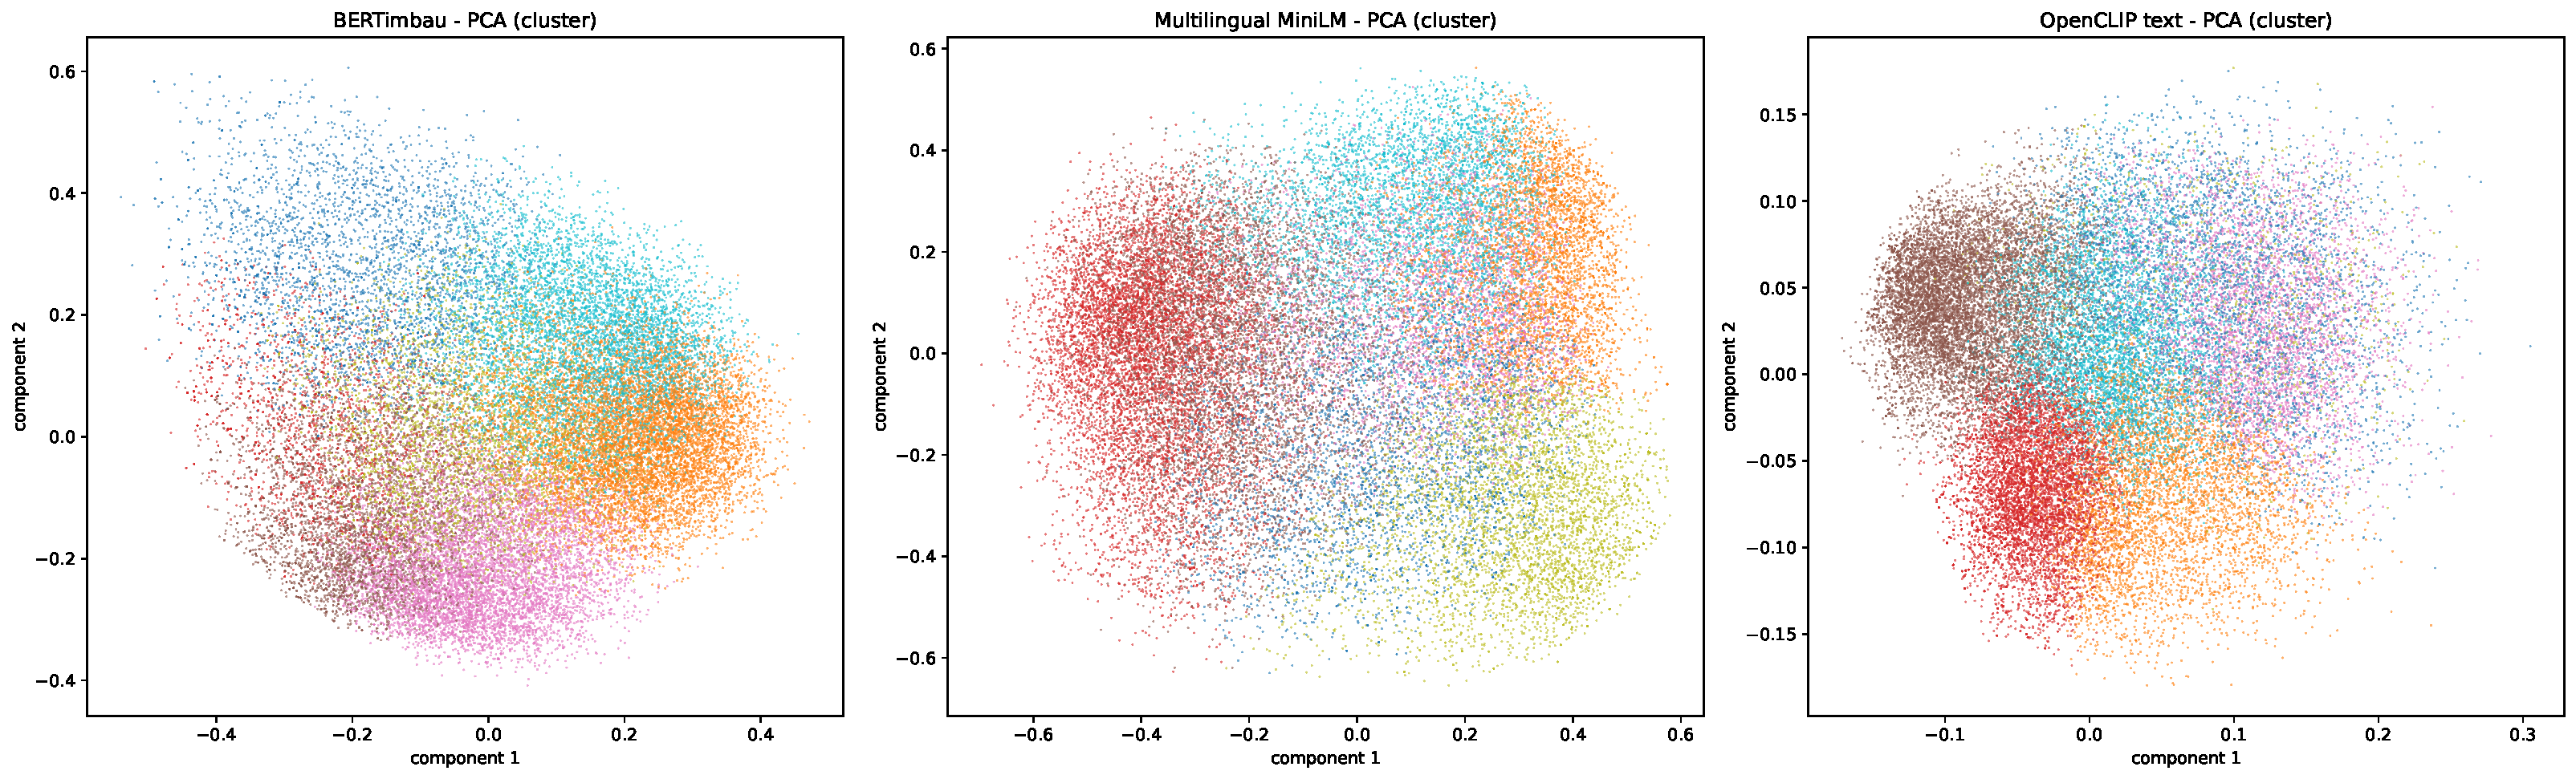
\includegraphics[width=0.98\textwidth]{olist_negative_sentiment_geometry_assets/figures/phase3_projection_pca_cluster.pdf}
\vspace{1mm}
{\footnotesize (a) PCA}\\[1mm]
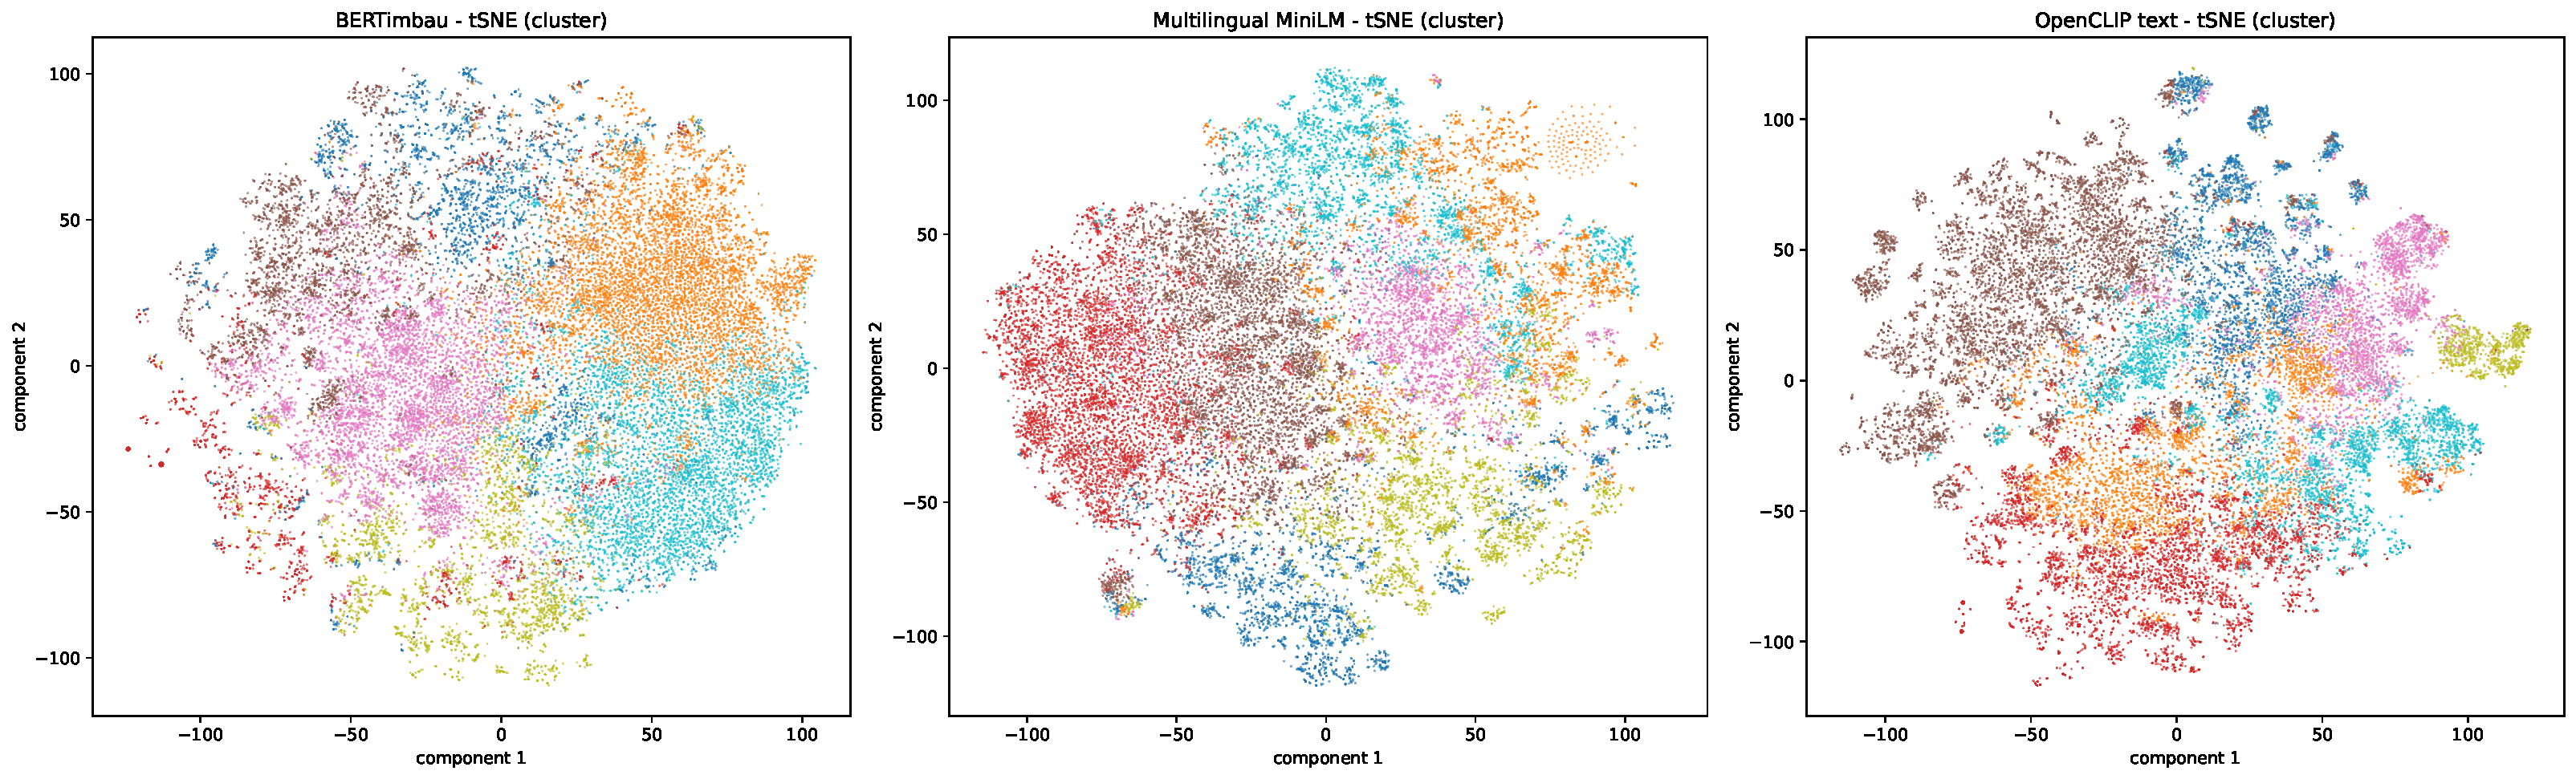
\includegraphics[width=0.98\textwidth]{olist_negative_sentiment_geometry_assets/figures/phase3_projection_tsne_cluster.pdf}
\vspace{1mm}
{\footnotesize (b) t-SNE}\\[1mm]
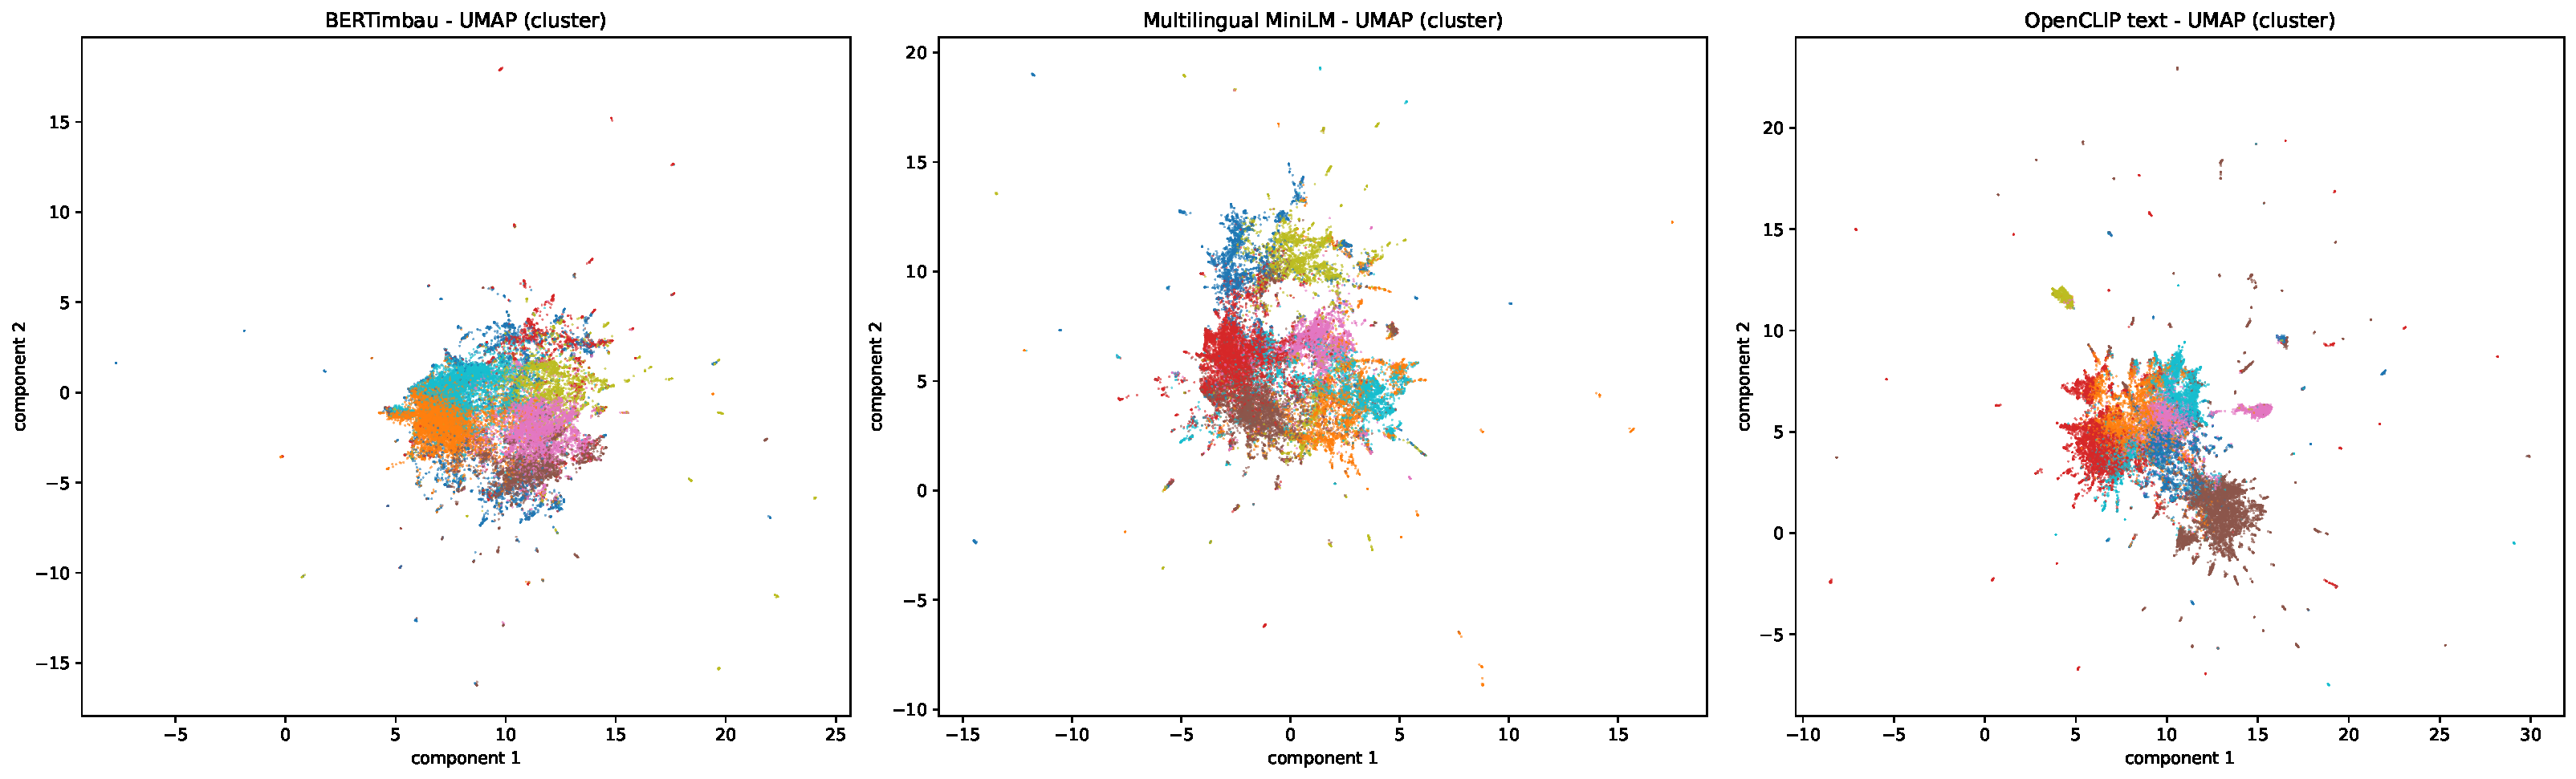
\includegraphics[width=0.98\textwidth]{olist_negative_sentiment_geometry_assets/figures/phase3_projection_umap_cluster.pdf}
\vspace{1mm}
{\footnotesize (c) UMAP}
\caption{Cross-method projection maps coloured by K-Means cluster ID (top-to-bottom: PCA, t-SNE, UMAP).}
\label{fig:phase3-projection-cluster-maps}
\end{figure*}

\begin{figure*}[tbp]
\centering
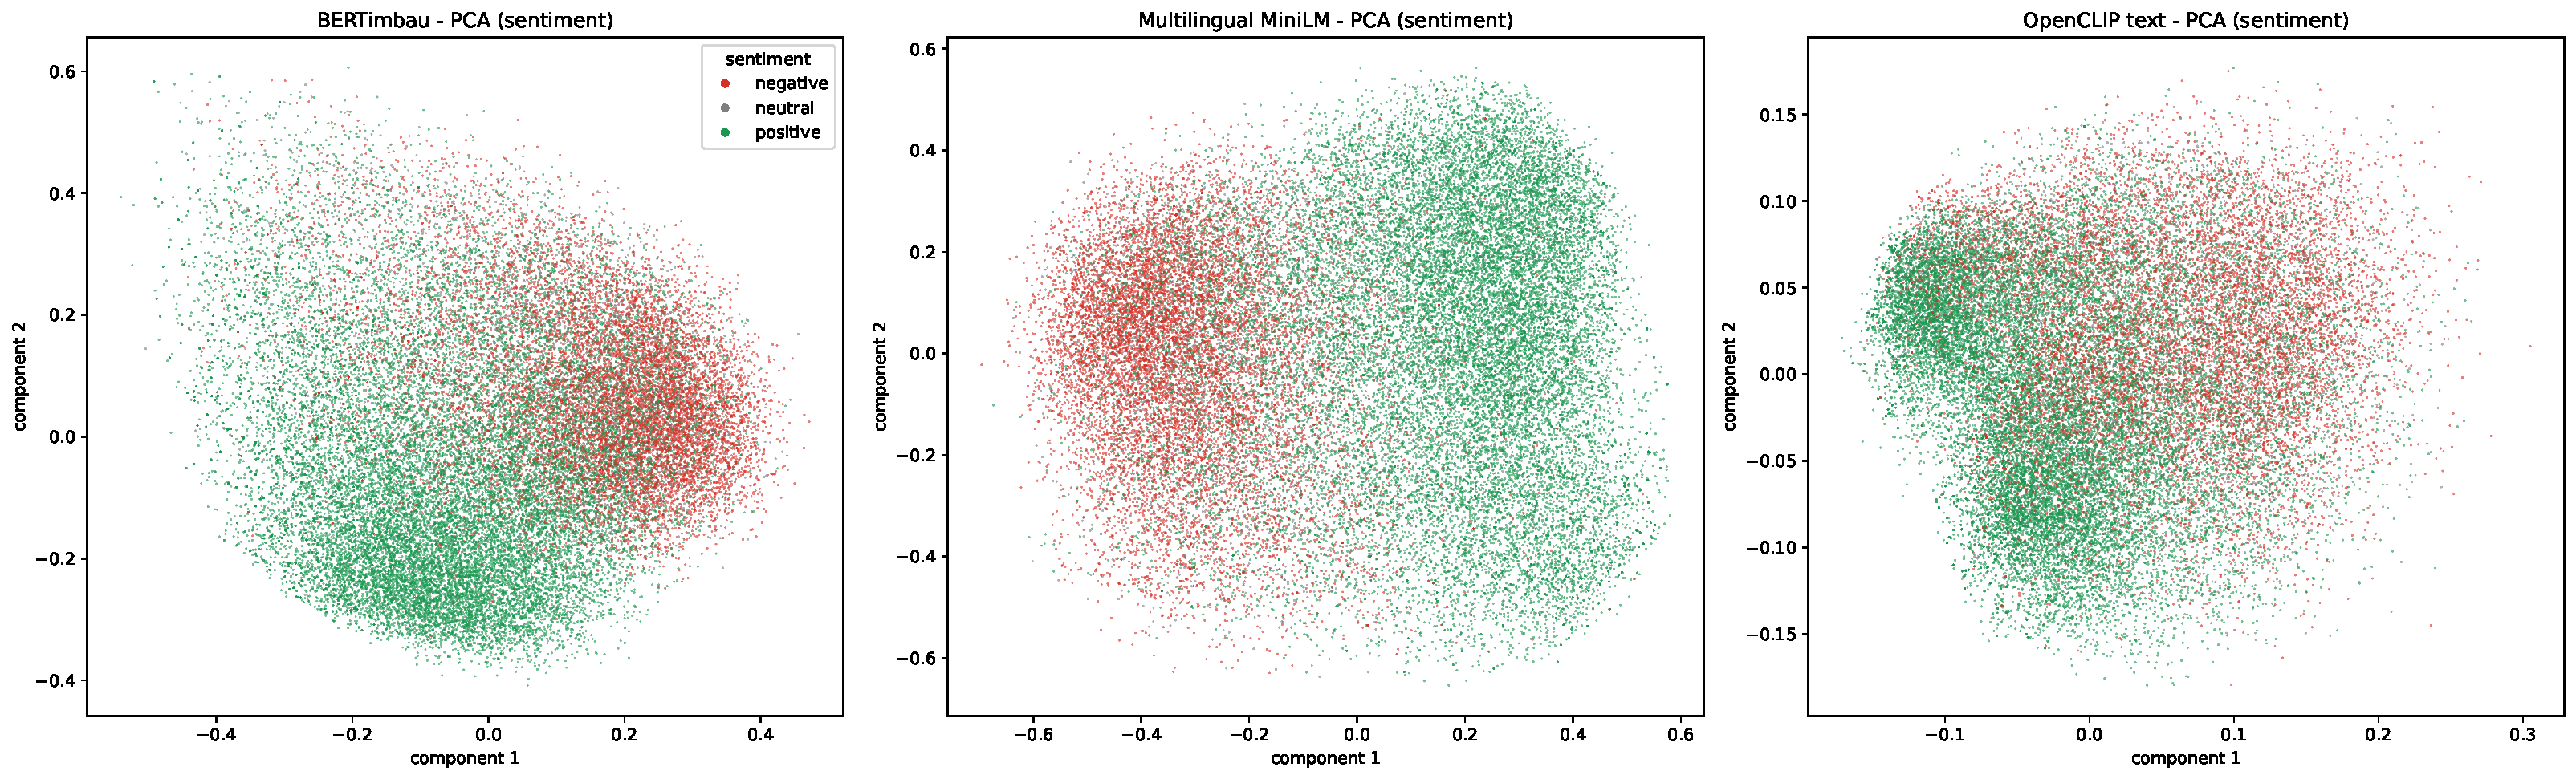
\includegraphics[width=0.98\textwidth]{olist_negative_sentiment_geometry_assets/figures/phase3_projection_pca_sentiment.pdf}
\vspace{1mm}
{\footnotesize (a) PCA}\\[1mm]
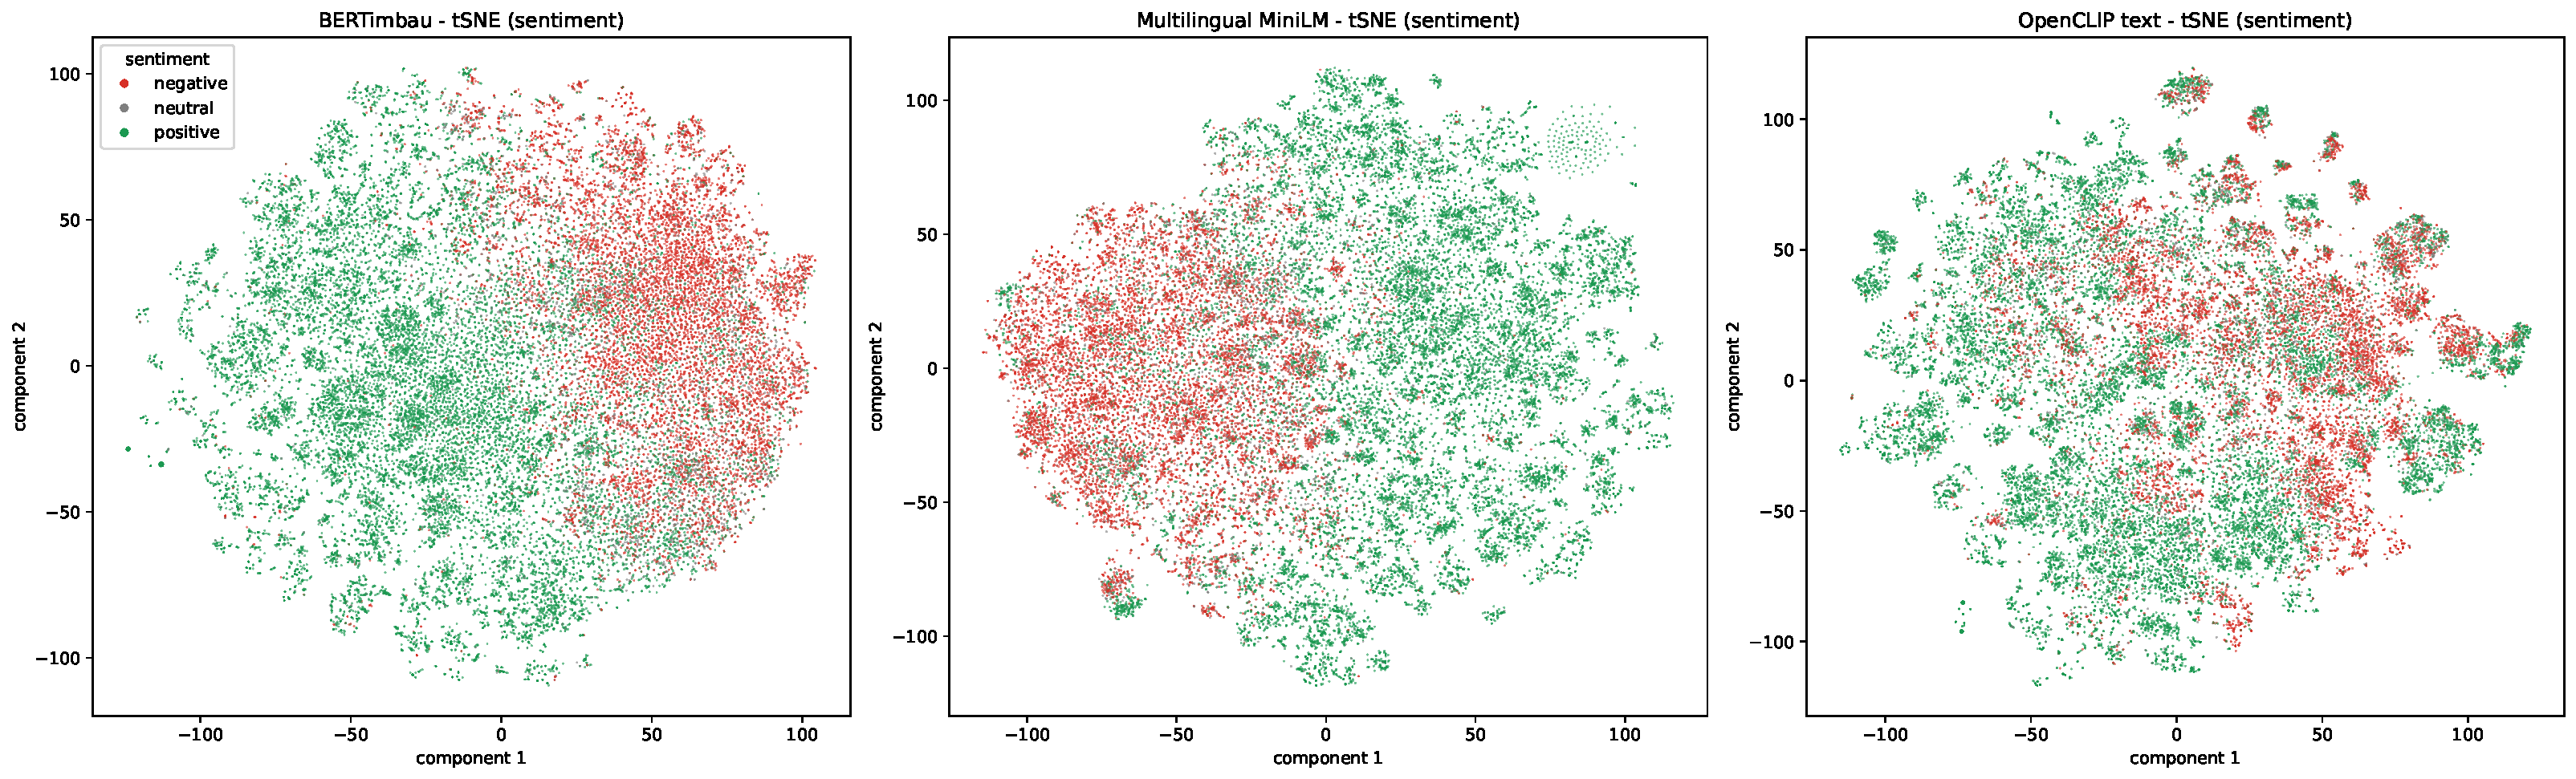
\includegraphics[width=0.98\textwidth]{olist_negative_sentiment_geometry_assets/figures/phase3_projection_tsne_sentiment.pdf}
\vspace{1mm}
{\footnotesize (b) t-SNE}\\[1mm]
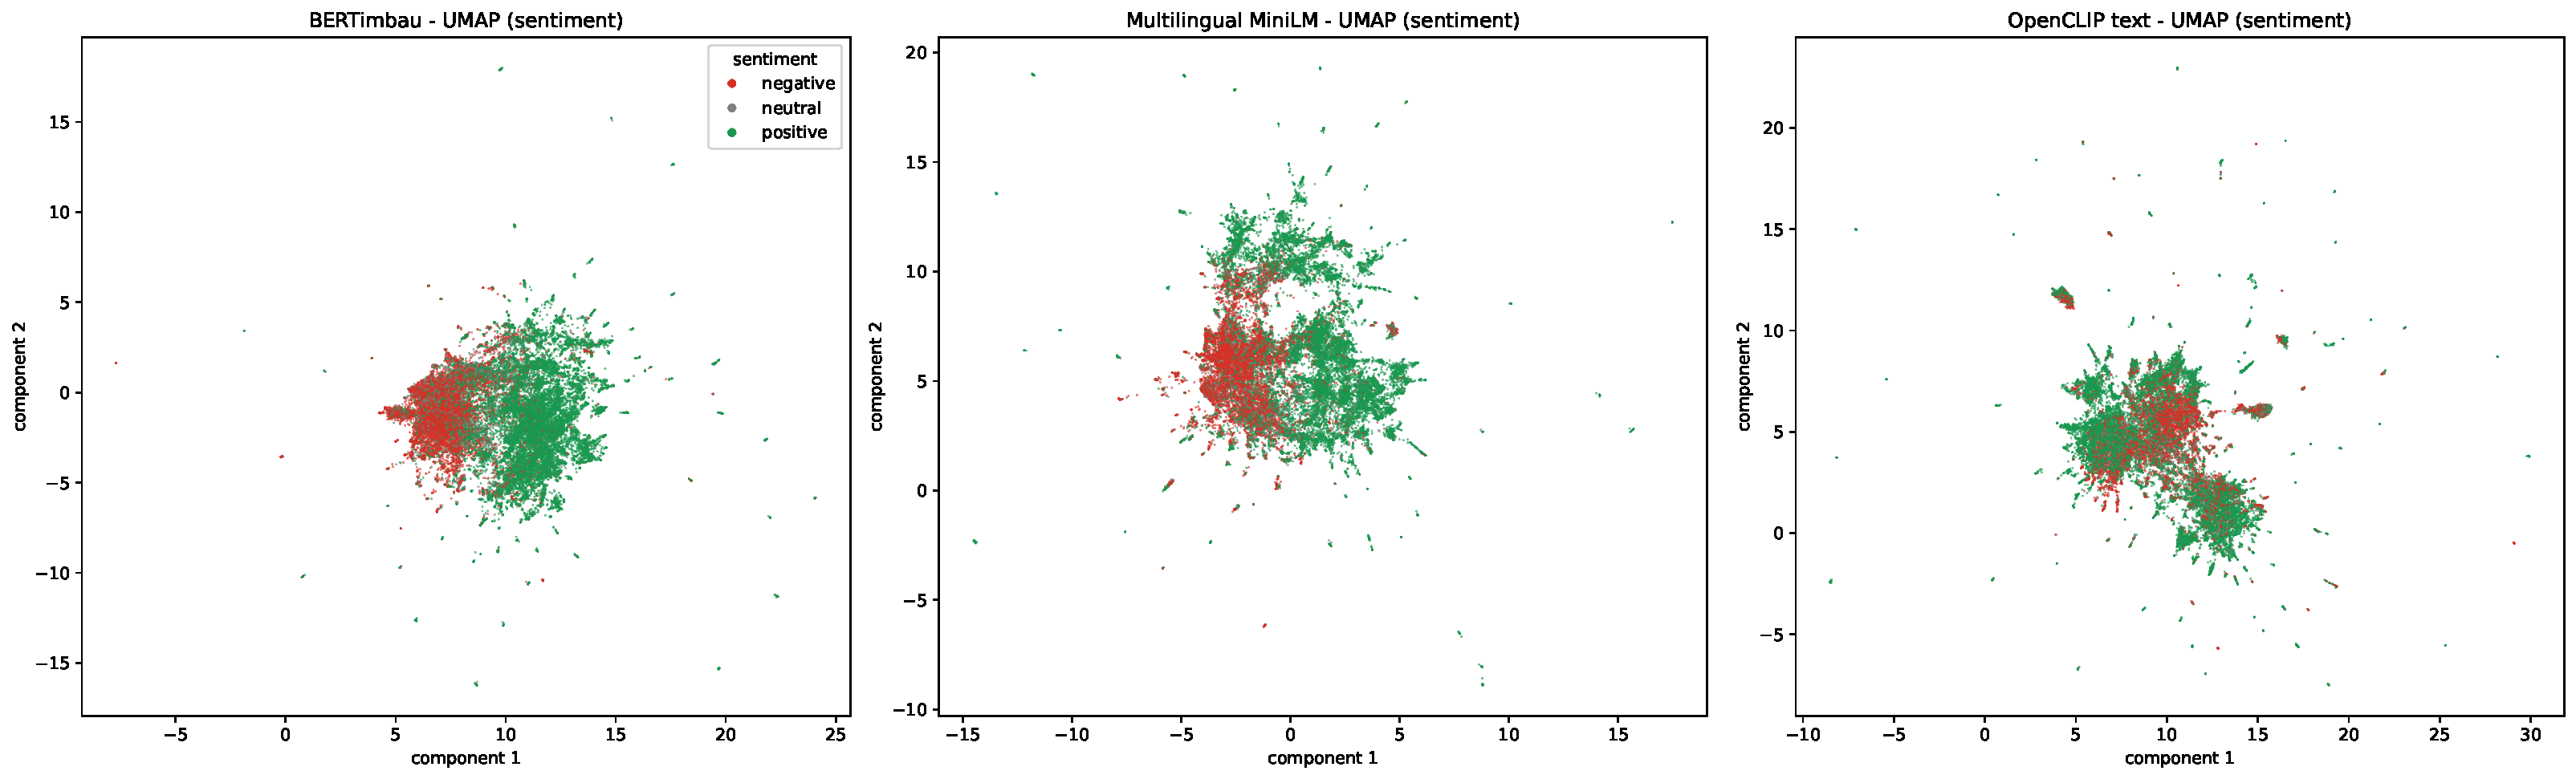
\includegraphics[width=0.98\textwidth]{olist_negative_sentiment_geometry_assets/figures/phase3_projection_umap_sentiment.pdf}
\vspace{1mm}
{\footnotesize (c) UMAP}
\caption{Cross-method projection maps coloured by sentiment group (\texttt{rating\_group}) (top-to-bottom: PCA, t-SNE, UMAP).}
\label{fig:phase3-projection-sentiment-maps}
\end{figure*}

\begin{figure*}[tbp]
\centering
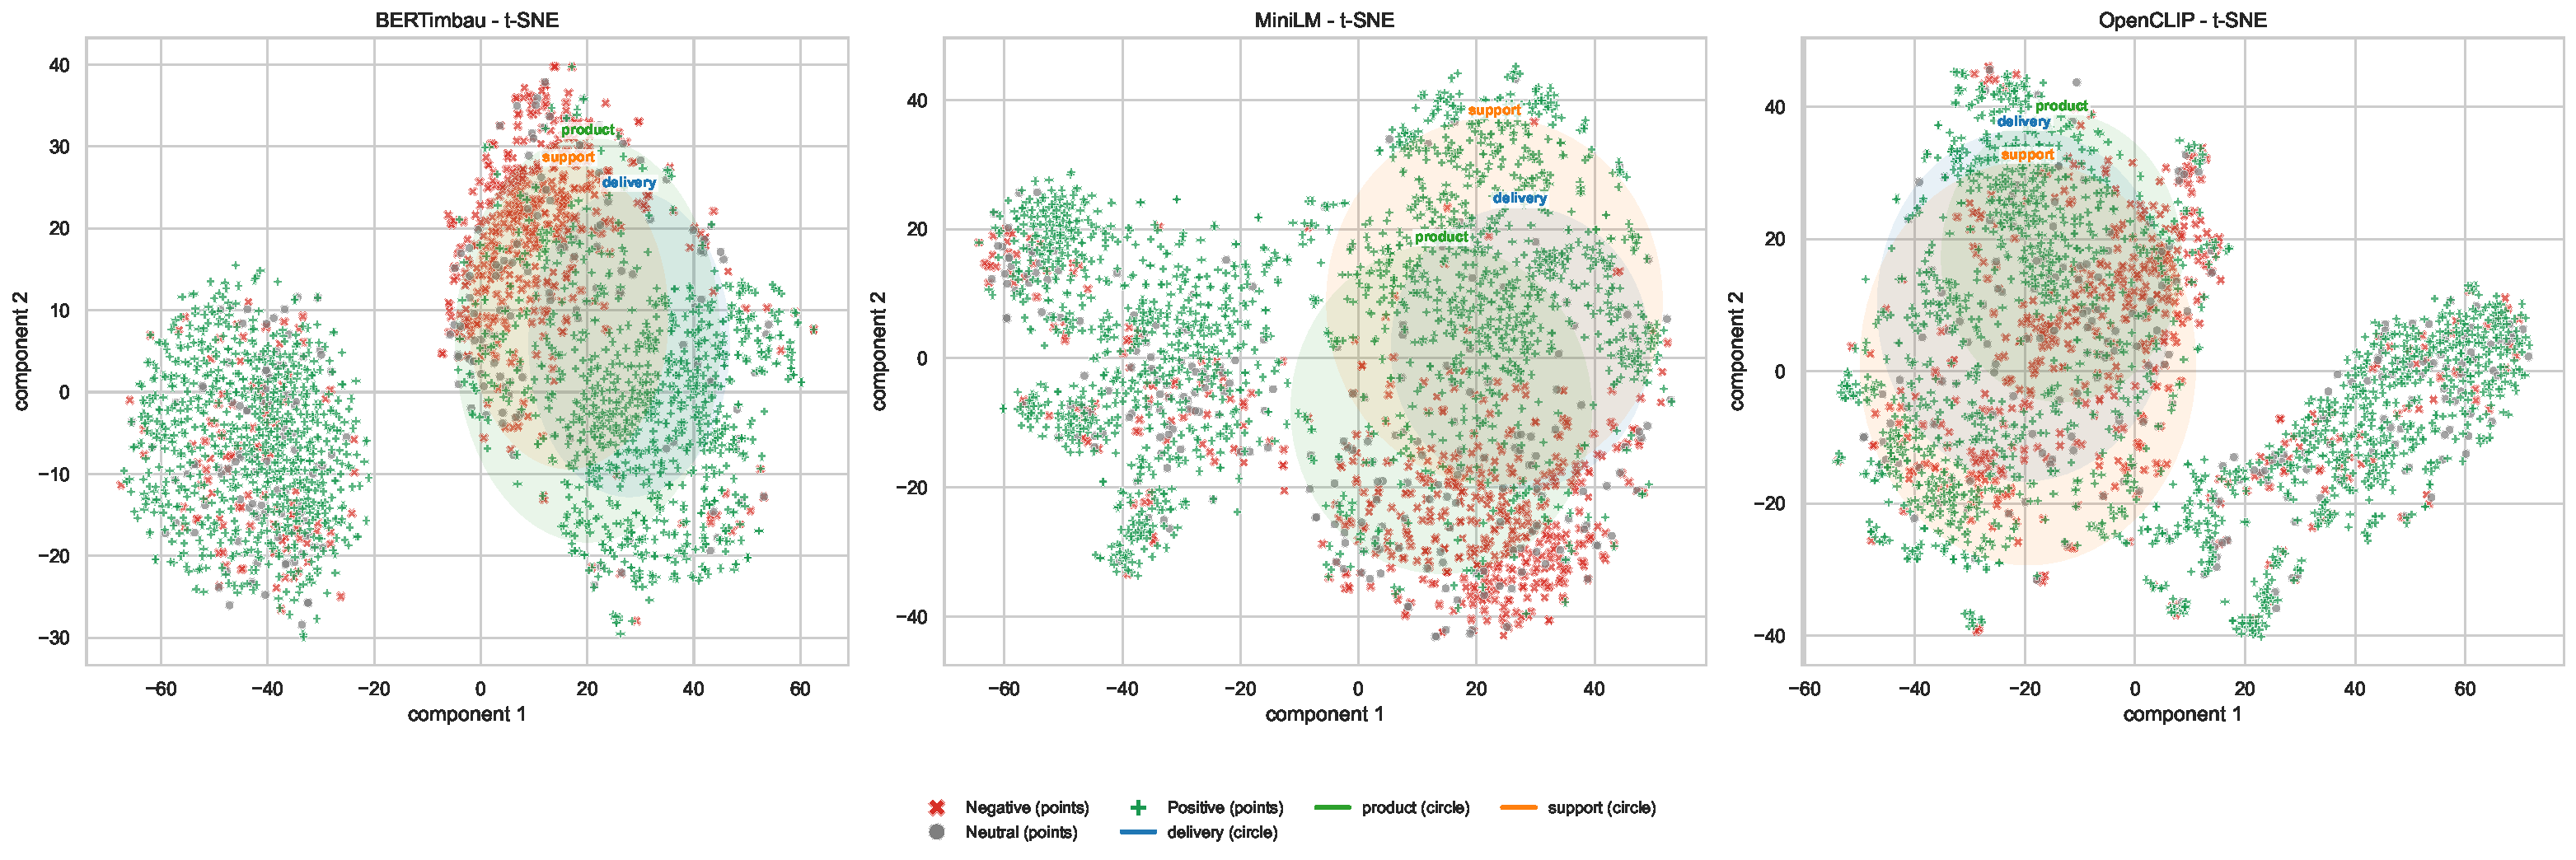
\includegraphics[width=0.98\textwidth]{olist_negative_sentiment_geometry_assets/figures/phase3_projection_tsne_sentiment_topic_circles.pdf}
\caption{t-SNE projections with sentiment-coloured points and topic-proxy circle overlays. Points encode sentiment; circle outlines summarise dominant service-topic regions (e.g., delivery, product, support) within each model space.}
\label{fig:phase3-tsne-sentiment-topic-circles}
\end{figure*}

\begin{figure}[tbp]
\centering
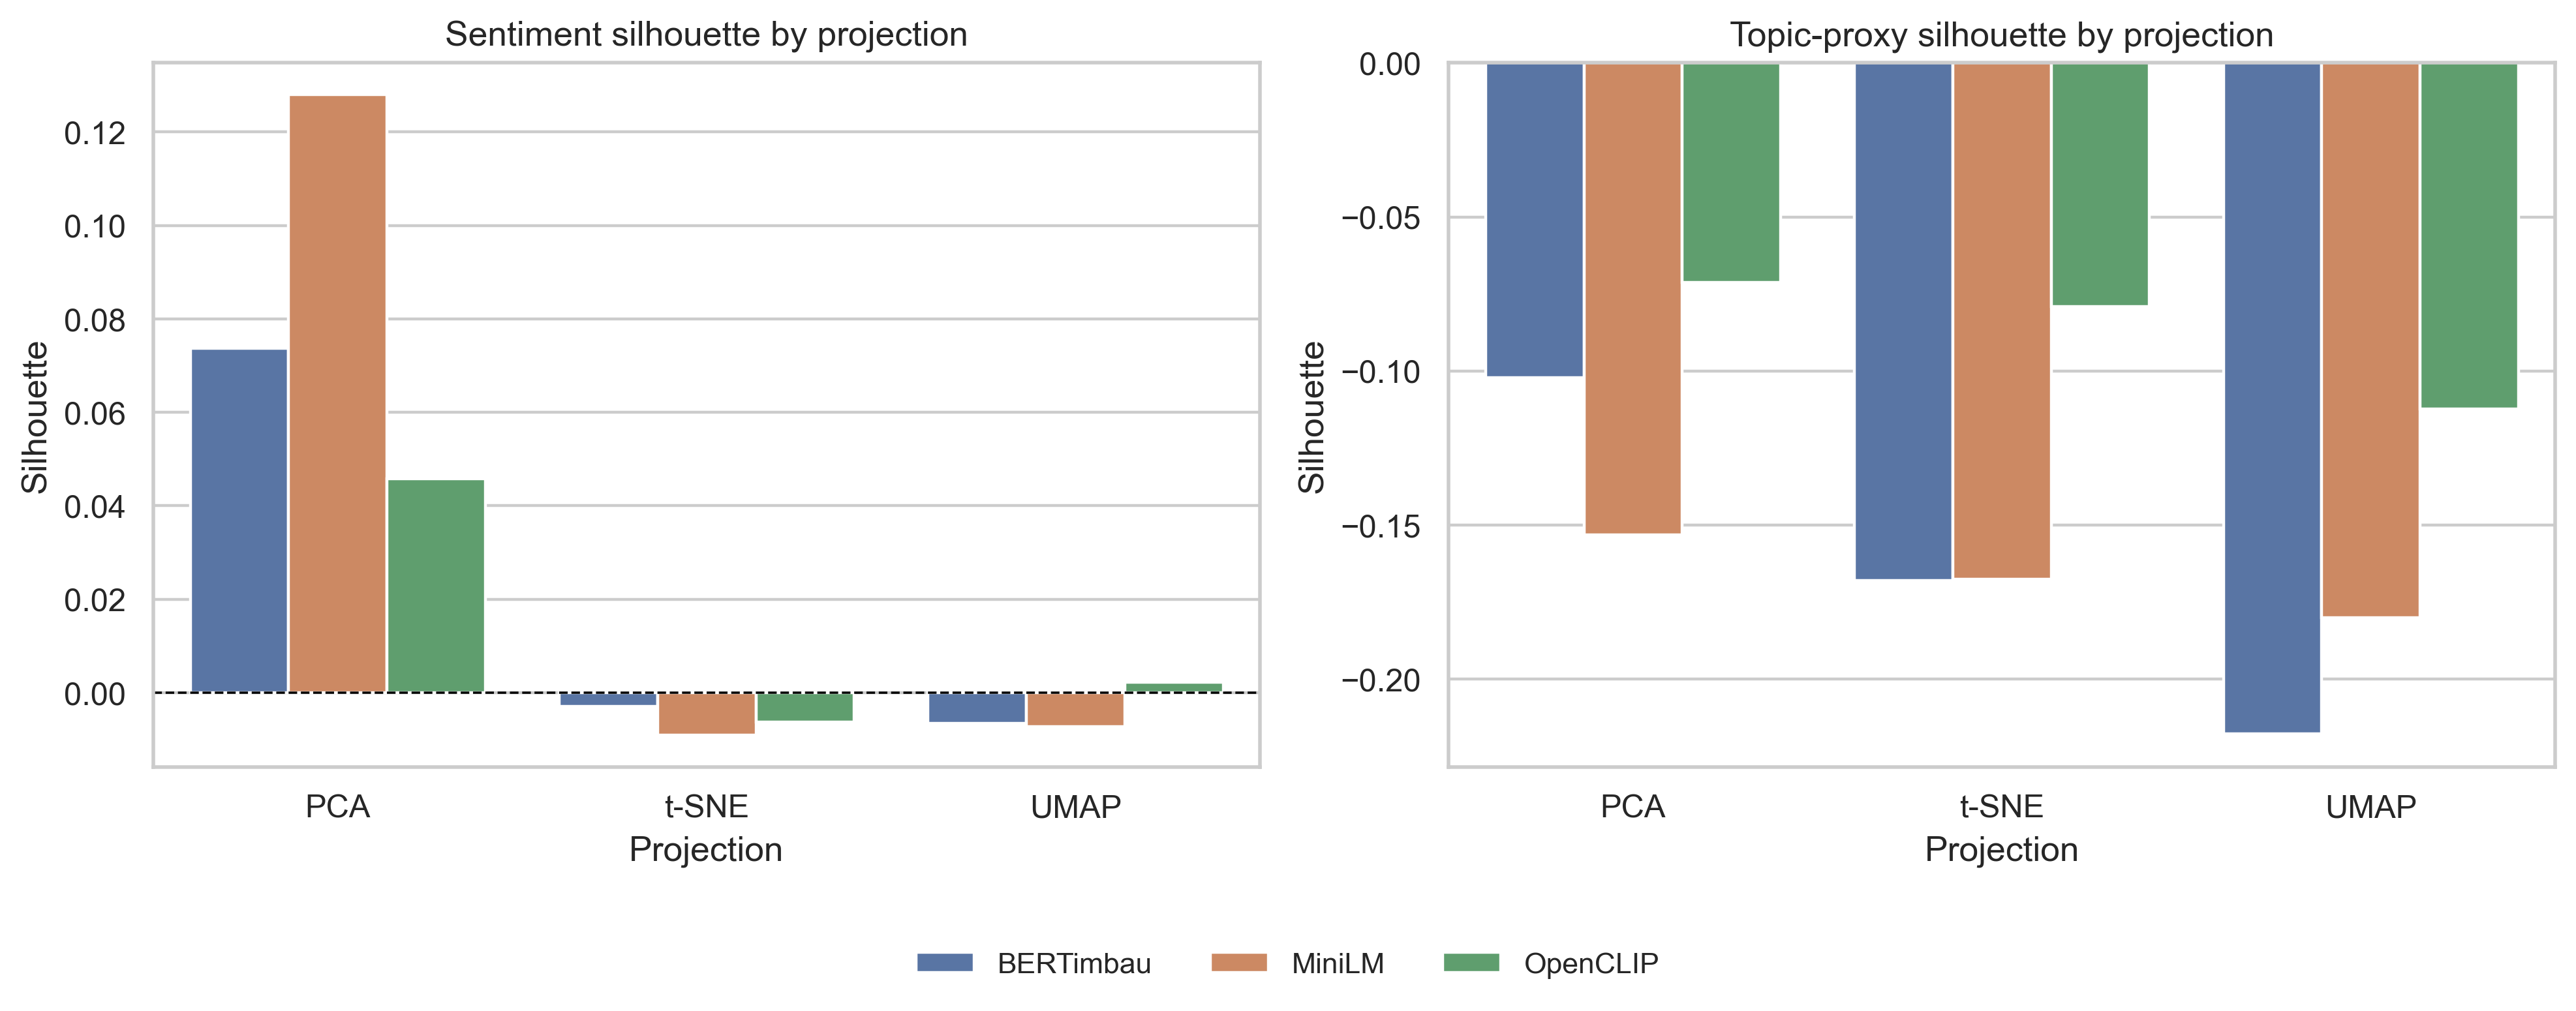
\includegraphics[width=\linewidth]{olist_negative_sentiment_geometry_assets/figures/phase3_projection_quality_sentiment_topic_absolute.png}
\caption{Absolute 2D silhouette values by projection method and model for sentiment labels (left) and topic-proxy labels (right).}
\label{fig:phase3-projection-quality-absolute}
\end{figure}

\begin{figure}[tbp]
\centering
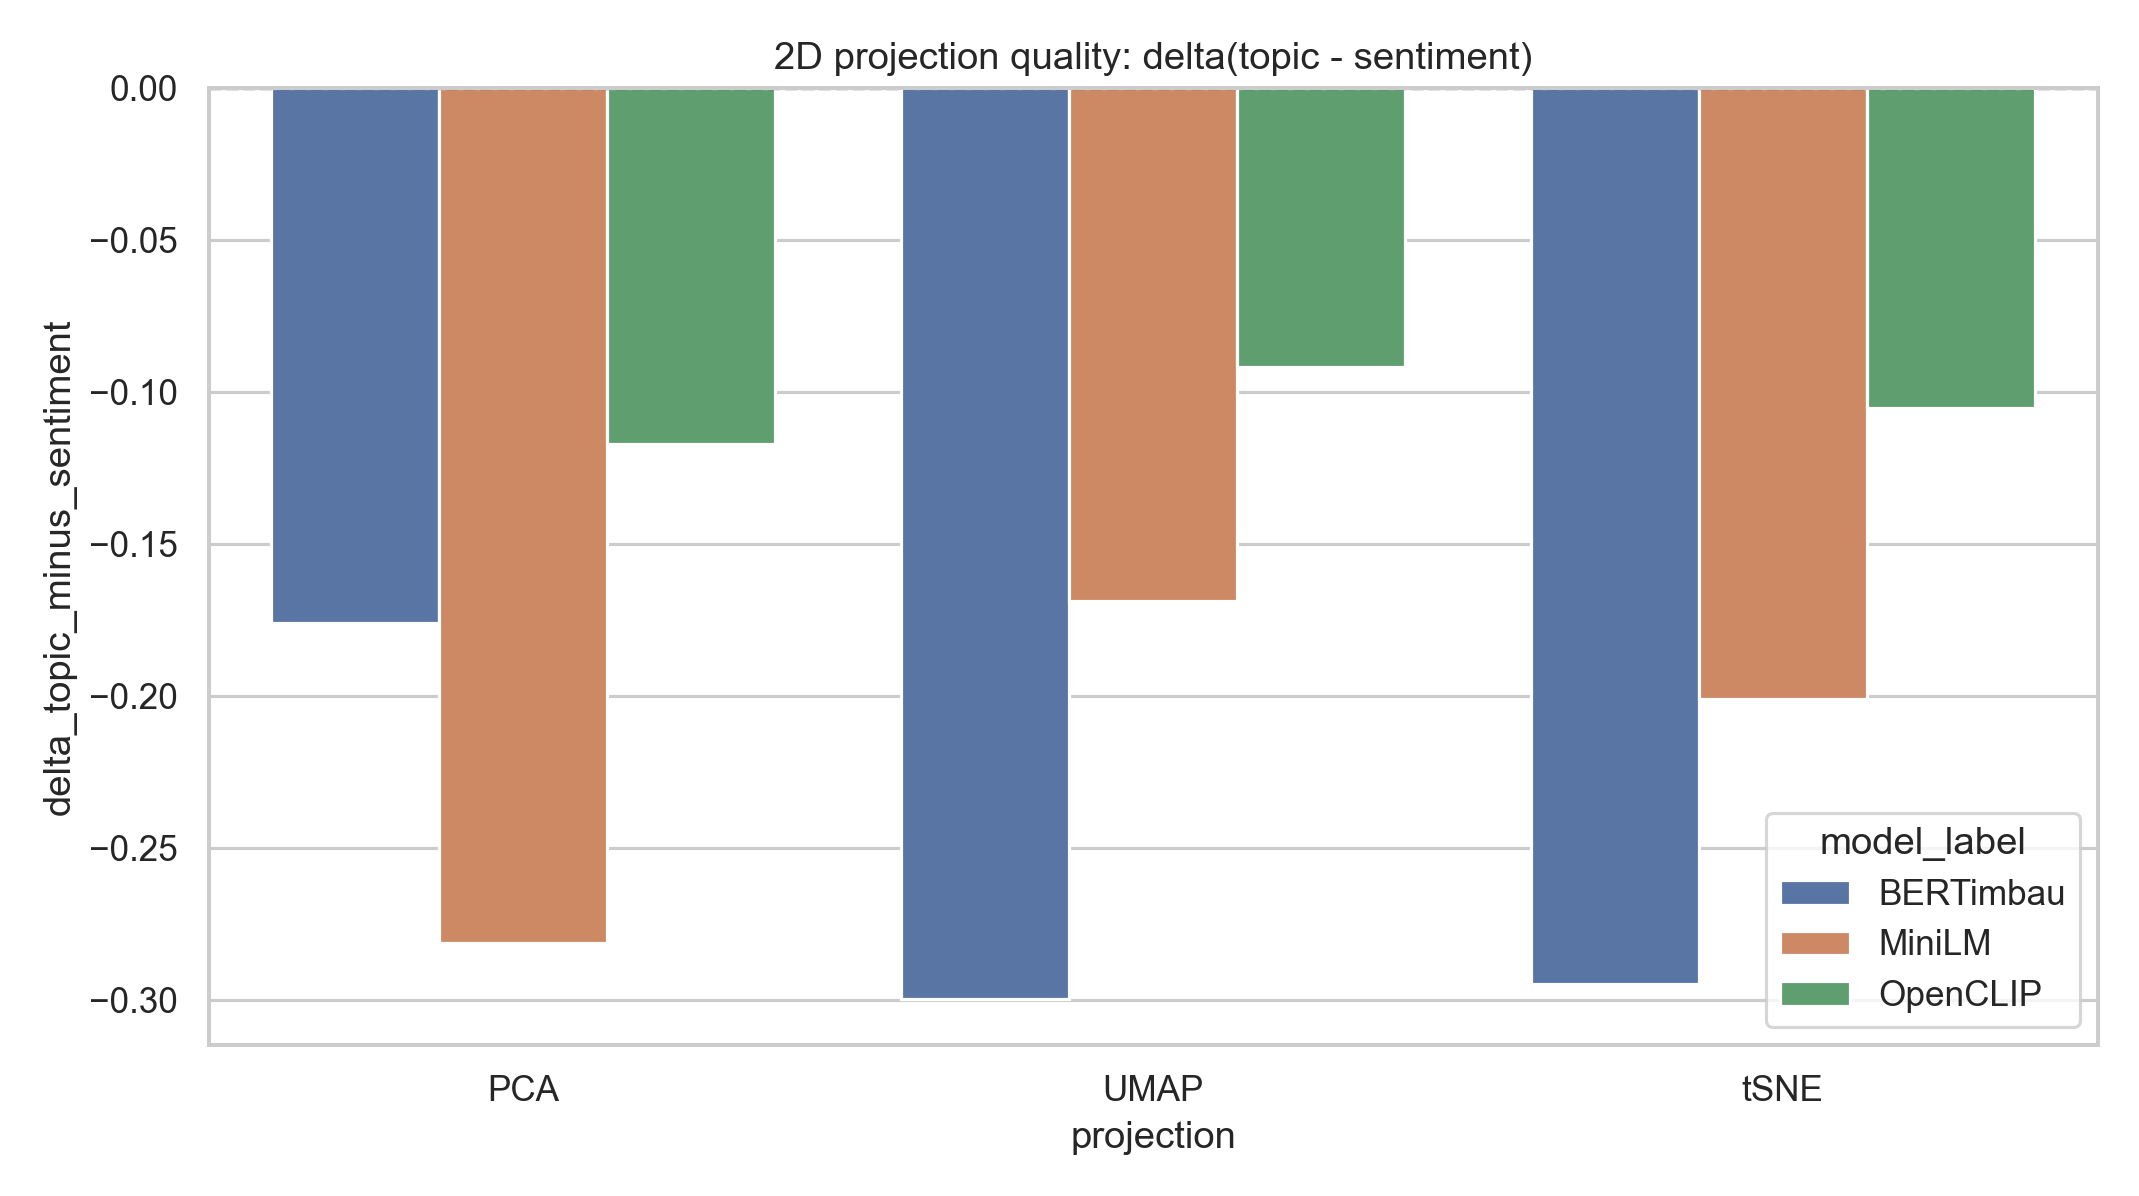
\includegraphics[width=\linewidth]{olist_negative_sentiment_geometry_assets/figures/phase3_projection_quality_delta_topic_minus_sentiment.png}
\caption{Projection quality comparison via $\Delta$ (topic silhouette minus sentiment silhouette). Negative values indicate stronger sentiment separation than topic separation in 2D maps.}
\label{fig:phase3-projection-quality-delta}
\end{figure}

\begin{table}[tbp]
\centering
\small
\caption{Exact $\Delta$ values for Figure~\ref{fig:phase3-projection-quality-delta} (topic silhouette minus sentiment silhouette).}
\label{tab:phase3-projection-delta-values}
\adjustbox{max width=\linewidth}{
\begin{tabular}{lccc}
\hline
\textbf{Model} & \textbf{PCA} & \textbf{t-SNE} & \textbf{UMAP} \\
\hline
BERTimbau & -0.176 & -0.295 & -0.300 \\
Multilingual MiniLM & -0.281 & -0.201 & -0.169 \\
OpenCLIP text & -0.117 & -0.105 & -0.092 \\
\hline
\end{tabular}
}
\end{table}

\subsection{Islandisation of Negative Reviews}

I now turn to the islandisation metrics introduced in Section~\ref{subsec:island-metrics}. 
The primary question (RQ1) is whether negative reviews form geometric islands or a diffuse layer within the seven-cluster structure.
Across models, negative reviews show partial islandisation: some dense, highly negative clusters coexist with a large diffuse layer spread across topics.

\paragraph{Cluster-wise negative ratios.}

Across models, the global share of negative reviews is $\bar{r} \approx 0.29$. 
In all three embedding spaces, the cluster-wise negative ratios $r_c$ vary substantially around this average: some clusters are heavily negative (ratios up to roughly 0.70--0.75), others are almost purely positive (ratios near 0.05--0.10), and a few are more balanced. 
The standard deviation $\sigma_r$ of these ratios is clearly above zero in every model ($\sigma_r \in [0.183, 0.287]$), showing that negativity is not evenly spread across clusters. 
This pattern already indicates partial islandisation: certain clusters act as negative ``hot spots'', while others are mostly positive.

\begin{figure}[tbp]
\centering
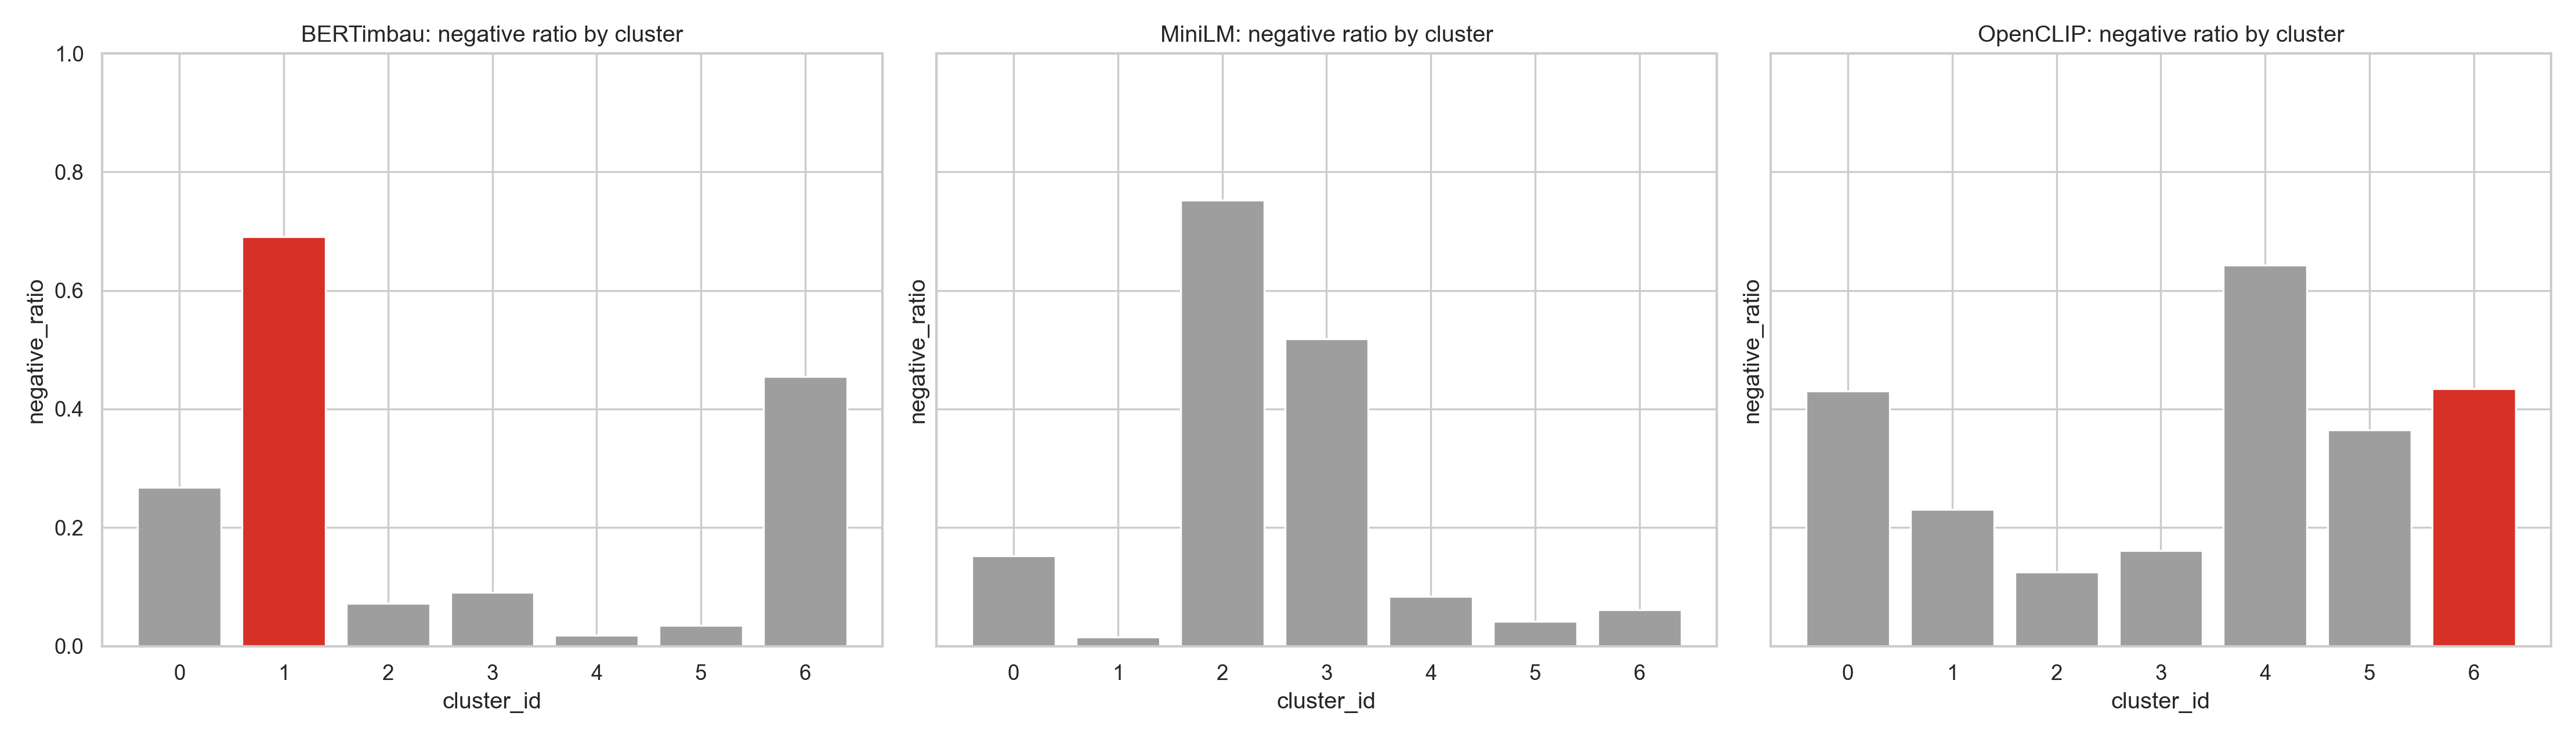
\includegraphics[width=\linewidth]{olist_negative_sentiment_geometry_assets/figures/phase4_negative_ratio_by_cluster_island_flag.png}
\caption{Negative ratio by cluster, with island flags based on high negative concentration and above-average density.}
\label{fig:phase4-negative-ratio-islands}
\end{figure}

\begin{figure}[tbp]
\centering
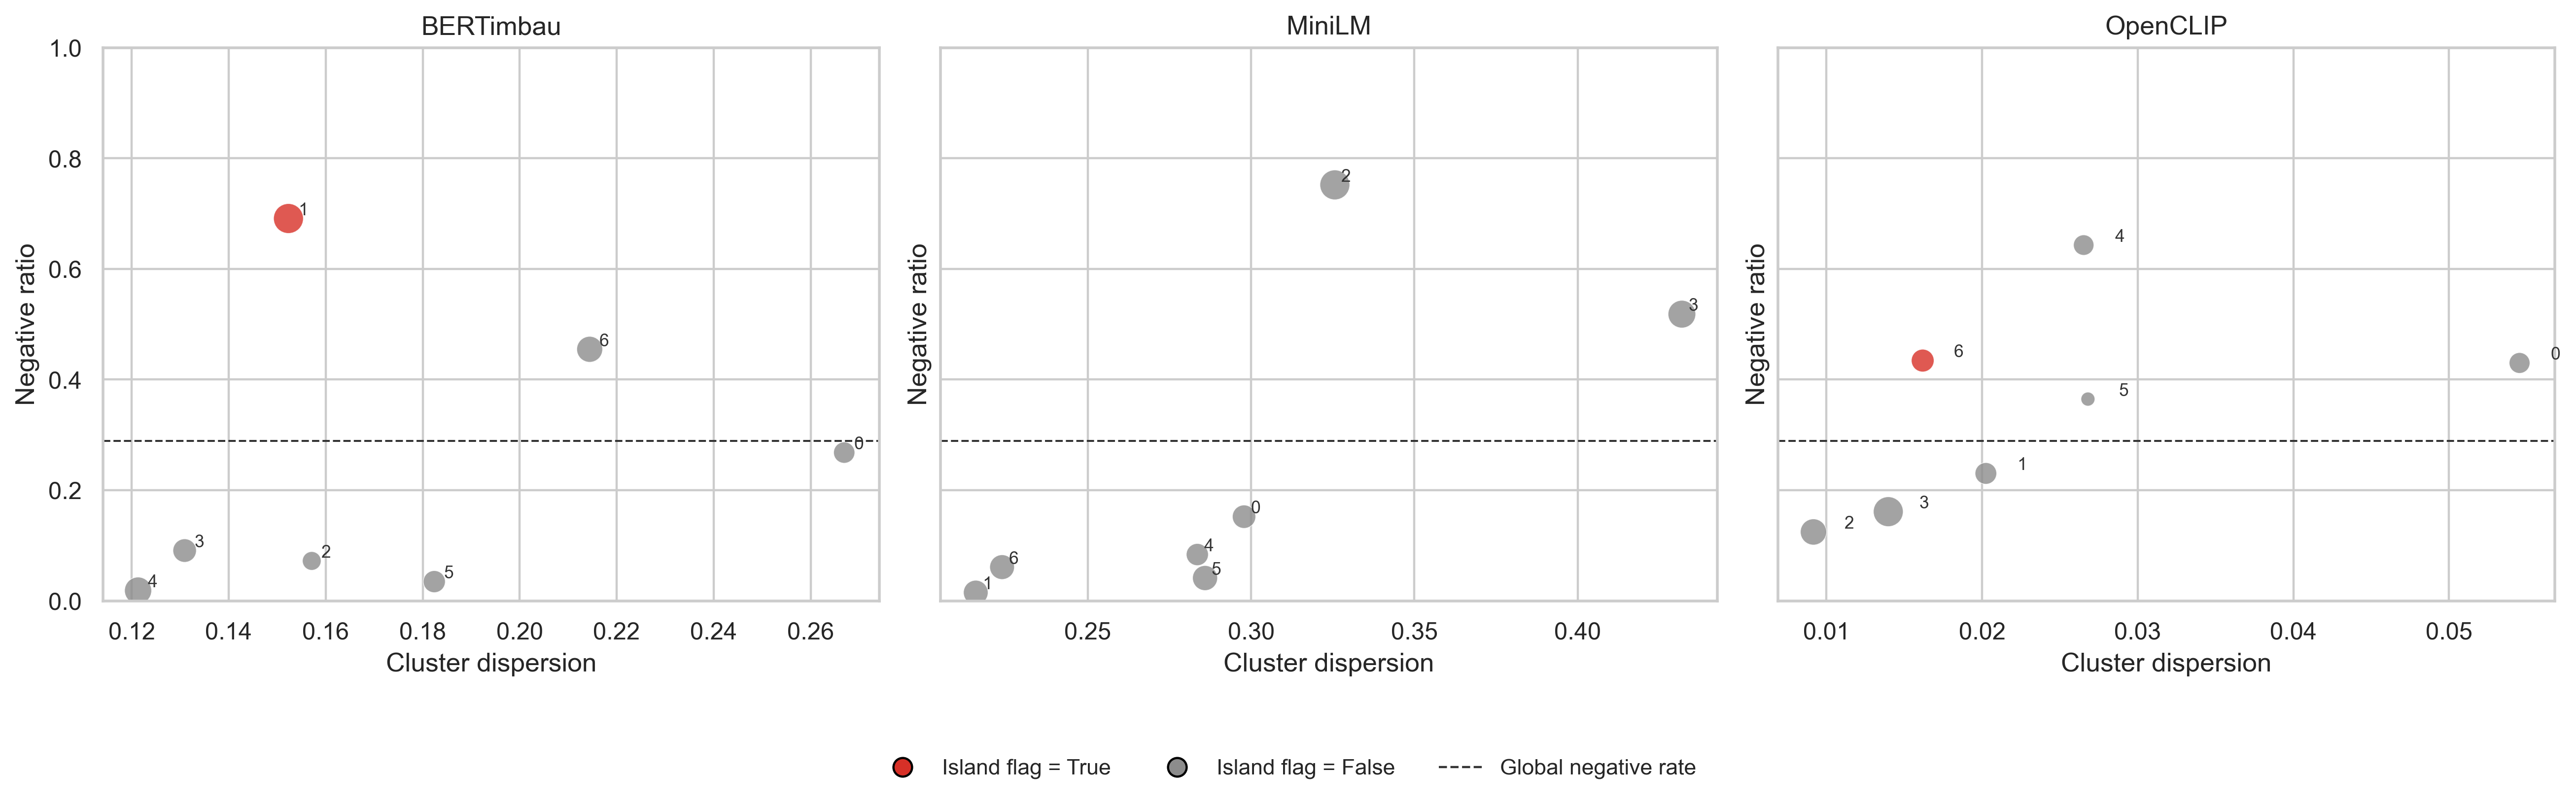
\includegraphics[width=\linewidth]{olist_negative_sentiment_geometry_assets/figures/phase4_island_criterion_scatter.png}
\caption{Island-criterion map by model: each point is a cluster with x = dispersion and y = negative ratio; red points satisfy the island flag.}
\label{fig:phase4-island-criterion-scatter}
\end{figure}

\paragraph{Negative homophily.}

The $k$-nearest neighbour graphs (with $k = 20$) show elevated negative homophily in all models. 
While the global negative rate is around 0.29, a typical negative review has between roughly 60\% and 70\% negative neighbours in BERTimbau and MiniLM, and somewhat lower but still elevated homophily in OpenCLIP. 
This means that negative reviews are more likely to be near other negatives than random chance would suggest, which is consistent with the presence of local negative regions.

\paragraph{Within-class dispersion.}

Within-class dispersion, measured by normalised average pairwise cosine distance, reveals that negative reviews are generally tighter than the corpus as a whole. 
For example, if the global average pairwise distance is normalised to 1.0, negative reviews tend to have dispersion values below 1 (for instance, around 0.8--0.9), whereas positive reviews are closer to the global baseline. 
This suggests that negative content often occupies more compact regions in embedding space, even though it is not confined to a single cluster.

\paragraph{Negative islands and diffuse components.}

Combining negative ratios and density, BERTimbau and OpenCLIP each exhibit one cluster that satisfies the negative-island criteria, while MiniLM has zero flagged islands under the same threshold rule. 
At the same time, MiniLM still shows strong negative concentration in specific clusters (for example, non-delivery and defective-product clusters), indicating unevenness without meeting the strict island flag definition. 
Qualitative inspection of high-negative clusters through regex-topic composition and exemplar reviews links them to intuitive complaint themes such as non-delivery or missing products, defective or incomplete items, and severe delays. 
Taken together, these results suggest that negative sentiment is neither purely islandised nor fully diffuse: discrete island flags appear in some models, while a sizeable diffuse layer of negative reviews remains interwoven with broader service themes.
These patterns answer RQ1 by showing that negative sentiment is neither uniformly diffuse nor confined to a single cluster, but manifests as both a few dense negative ``hot spots'' and a broader diffuse layer.

\subsection{Model Comparison of Islandisation}

The second research question (RQ2) asks how the strength and shape of negative islandisation differ across the three embedding families.

Table~\ref{tab:phase4-model-comparison} provides the main cross-model islandisation profile.

\begin{table}[tbp]
\centering
\small
\caption{Main islandisation metrics by embedding model.}
\label{tab:phase4-model-comparison}
\adjustbox{max width=\linewidth}{
\begin{tabular}{lcccccc}
\hline
\textbf{Model} & \textbf{$\sigma_r$} & \textbf{95\% CI ($\sigma_r$)} & \textbf{Neg. homophily} & \textbf{Islands} & \textbf{Island mass} & \textbf{RQ1 label} \\
\hline
BERTimbau & 0.256 & [0.252, 0.259] & 0.725 & 1 & 0.234 & islands \\
MiniLM    & 0.287 & [0.283, 0.290] & 0.703 & 0 & 0.000 & diffuse \\
OpenCLIP  & 0.183 & [0.178, 0.188] & 0.595 & 1 & 0.144 & islands \\
\hline
\end{tabular}
}
\end{table}

\paragraph{Cluster-level dispersion of negative ratios.}

Bootstrap analysis of the standard deviation of cluster-wise negative ratios $\sigma_r$ shows systematic differences between models: Multilingual MiniLM has the highest $\sigma_r$ (0.287), BERTimbau is slightly lower (0.256), and OpenCLIP has the lowest (0.183), each with tight confidence intervals (Table~\ref{tab:phase4-model-comparison}). 
Pairwise bootstrap comparisons indicate that the differences between MiniLM and OpenCLIP, and between BERTimbau and OpenCLIP, are well above zero with high confidence, while the difference between MiniLM and BERTimbau is smaller but still noticeable. 
This suggests that MiniLM and BERTimbau produce more uneven negative ratios across clusters than OpenCLIP, consistent with stronger negative concentration.

\paragraph{Negative island count and mass.}

Using the island definition based on both $r_c$ and density, BERTimbau and OpenCLIP each yield one cluster that qualifies as a negative island, whereas MiniLM yields zero flagged islands. 
Measured as a share of all reviews, island mass is 0.234 for BERTimbau, 0.000 for MiniLM, and 0.144 for OpenCLIP. 
Hence, MiniLM’s high $\sigma_r$ reflects diffuse concentration across multiple negative-heavy clusters rather than concentration inside a single dense island cluster.

\paragraph{Homophily and dispersion across models.}

BERTimbau generally shows the strongest local negative homophily, suggesting that when negatives do cluster, they form tight groups in its space. 
MiniLM balances high sentiment purity with somewhat more diffuse negative spread, implying that it captures sentiment cleanly at the cluster level without collapsing all negative content into a single region. 
OpenCLIP exhibits lower sentiment purity and homophily and higher within-class dispersion for negatives, consistent with its cross-modal training objective and a geometry that is less specialised for polarity.

\begin{table}[tbp]
\centering
\small
\caption{Bootstrap pairwise contrasts for $\sigma_r$ (400 resamples, 95\% CI).}
\label{tab:phase4-bootstrap-rq2}
\adjustbox{max width=\linewidth}{
\begin{tabular}{lccc}
\hline
\textbf{Model pair} & \textbf{$\Delta$ mean} & \textbf{95\% CI} & \textbf{Stronger} \\
\hline
BERTimbau -- MiniLM & -0.031 & [-0.034, -0.028] & MiniLM \\
BERTimbau -- OpenCLIP & 0.073 & [0.069, 0.078] & BERTimbau \\
MiniLM -- OpenCLIP & 0.104 & [0.100, 0.109] & MiniLM \\
\hline
\end{tabular}
}
\end{table}

\noindent\textit{Interpretation note:} deltas are defined as $\Delta=\sigma_r^{\text{Model A}}-\sigma_r^{\text{Model B}}$; positive values indicate stronger cluster-level negative-ratio unevenness (more island-like concentration) in Model A.

\begin{figure}[tbp]
\centering
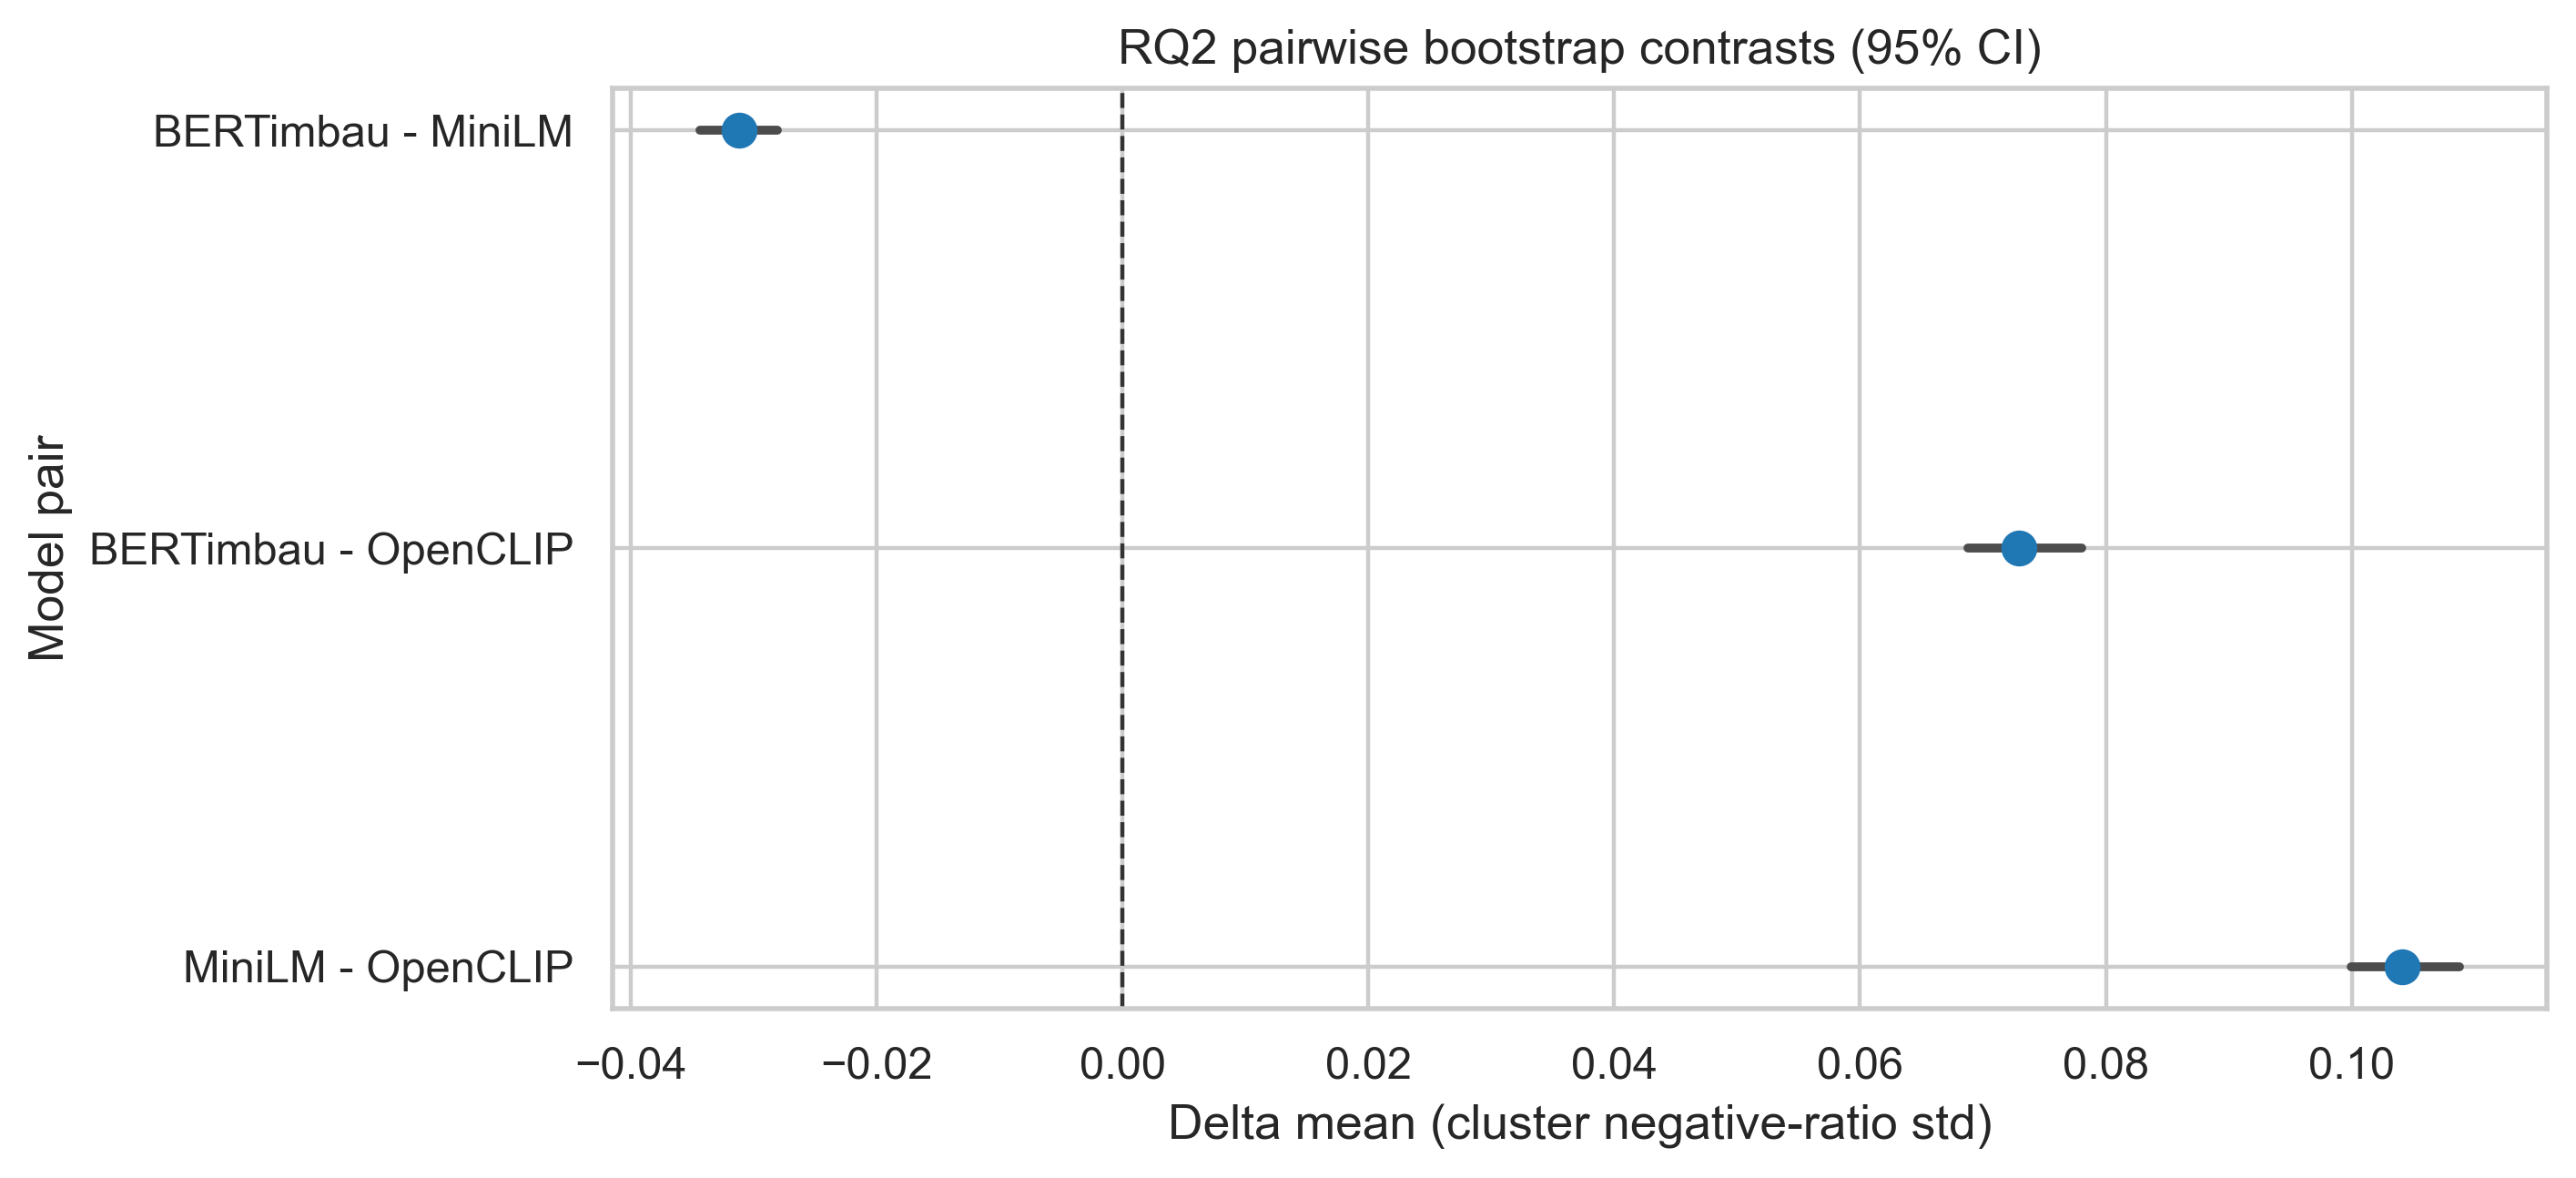
\includegraphics[width=\linewidth]{olist_negative_sentiment_geometry_assets/figures/phase4_rq2_pairwise_delta_forest.png}
\caption{RQ2 pairwise bootstrap contrasts for $\sigma_r$: points are mean deltas and horizontal segments are 95\% confidence intervals.}
\label{fig:phase4-rq2-forest}
\end{figure}

\paragraph{Summary for RQ2.}

Overall, the islandisation metrics and bootstrap comparisons indicate that all three models encode some form of negative concentration, but with different strengths and patterns. 
Bootstrap deltas show that BERTimbau has significantly higher $\sigma_r$ than OpenCLIP, and MiniLM has significantly higher $\sigma_r$ than OpenCLIP; MiniLM is also slightly but consistently higher than BERTimbau. 
At the same time, MiniLM spreads negativity across several thematically coherent clusters and is classified as diffuse under the strict island-flag rule, whereas BERTimbau tends to form tighter negative pockets with one flagged island. 
OpenCLIP, in contrast, yields more sentiment-mixed clusters and weaker islandisation, reflecting a geometry that is less aligned with review sentiment. 
These differences answer RQ2 by showing that BERTimbau and MiniLM encode stronger cluster-level unevenness than OpenCLIP, and that MiniLM’s negativity is more diffusely concentrated across multiple clusters.

The bootstrap contrasts that support this conclusion are reported in Table~\ref{tab:phase4-bootstrap-rq2}.


\subsection{k-NN and Local Neighbourhoods}
\label{subsec:knn-results}

To complement the global cluster analysis, I examine local neighbourhoods in each embedding space using $k$-nearest neighbours with $k = 20$ (Figure~\ref{fig:knn-neighbourhoods}). 
I use one fixed ambiguous delivery anchor (\textit{``o produto chegou no prazo mas recusei no ato da entrega por motivos de desistência''}), retrieve its 20 nearest neighbours in each embedding model with cosine distance over $\ell_2$-normalised vectors, and project the 21 local points (anchor + neighbours) to 2D with PCA for readability.

\begin{figure*}[tbp]
\centering
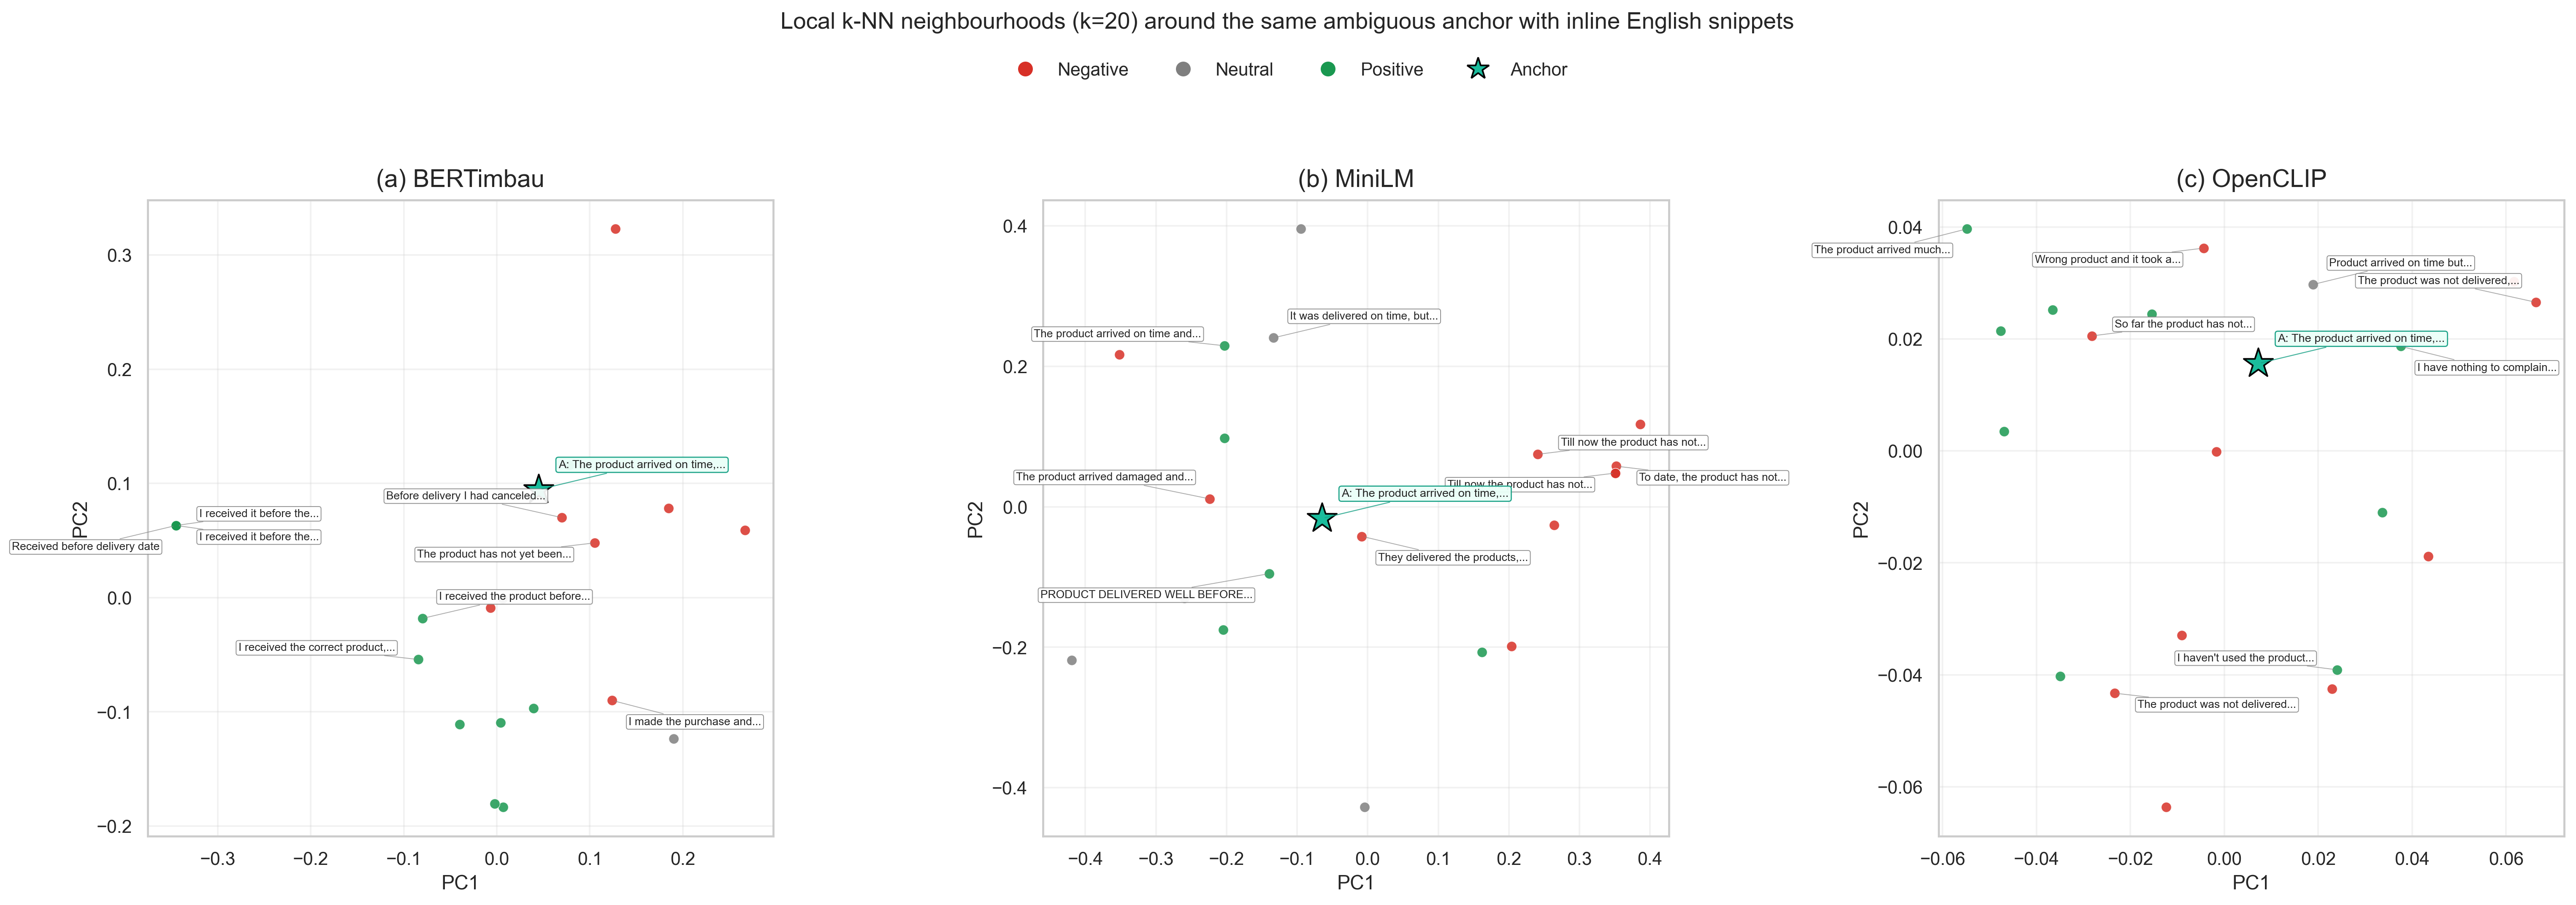
\includegraphics[width=0.98\textwidth]{olist_negative_sentiment_geometry_assets/figures/phase3_knn_neighbourhoods_anchor_ambiguous_k20_en.png}
\caption{Local $k$-NN neighbourhoods ($k=20$) for one ambiguous delivery anchor across embedding models: (a) BERTimbau, (b) Multilingual MiniLM, and (c) OpenCLIP text. Points are coloured by sentiment and the anchor is highlighted; numbered points are linked to English snippets below each panel.}
\label{fig:knn-neighbourhoods}
\end{figure*}

\begin{figure}[tbp]
\centering
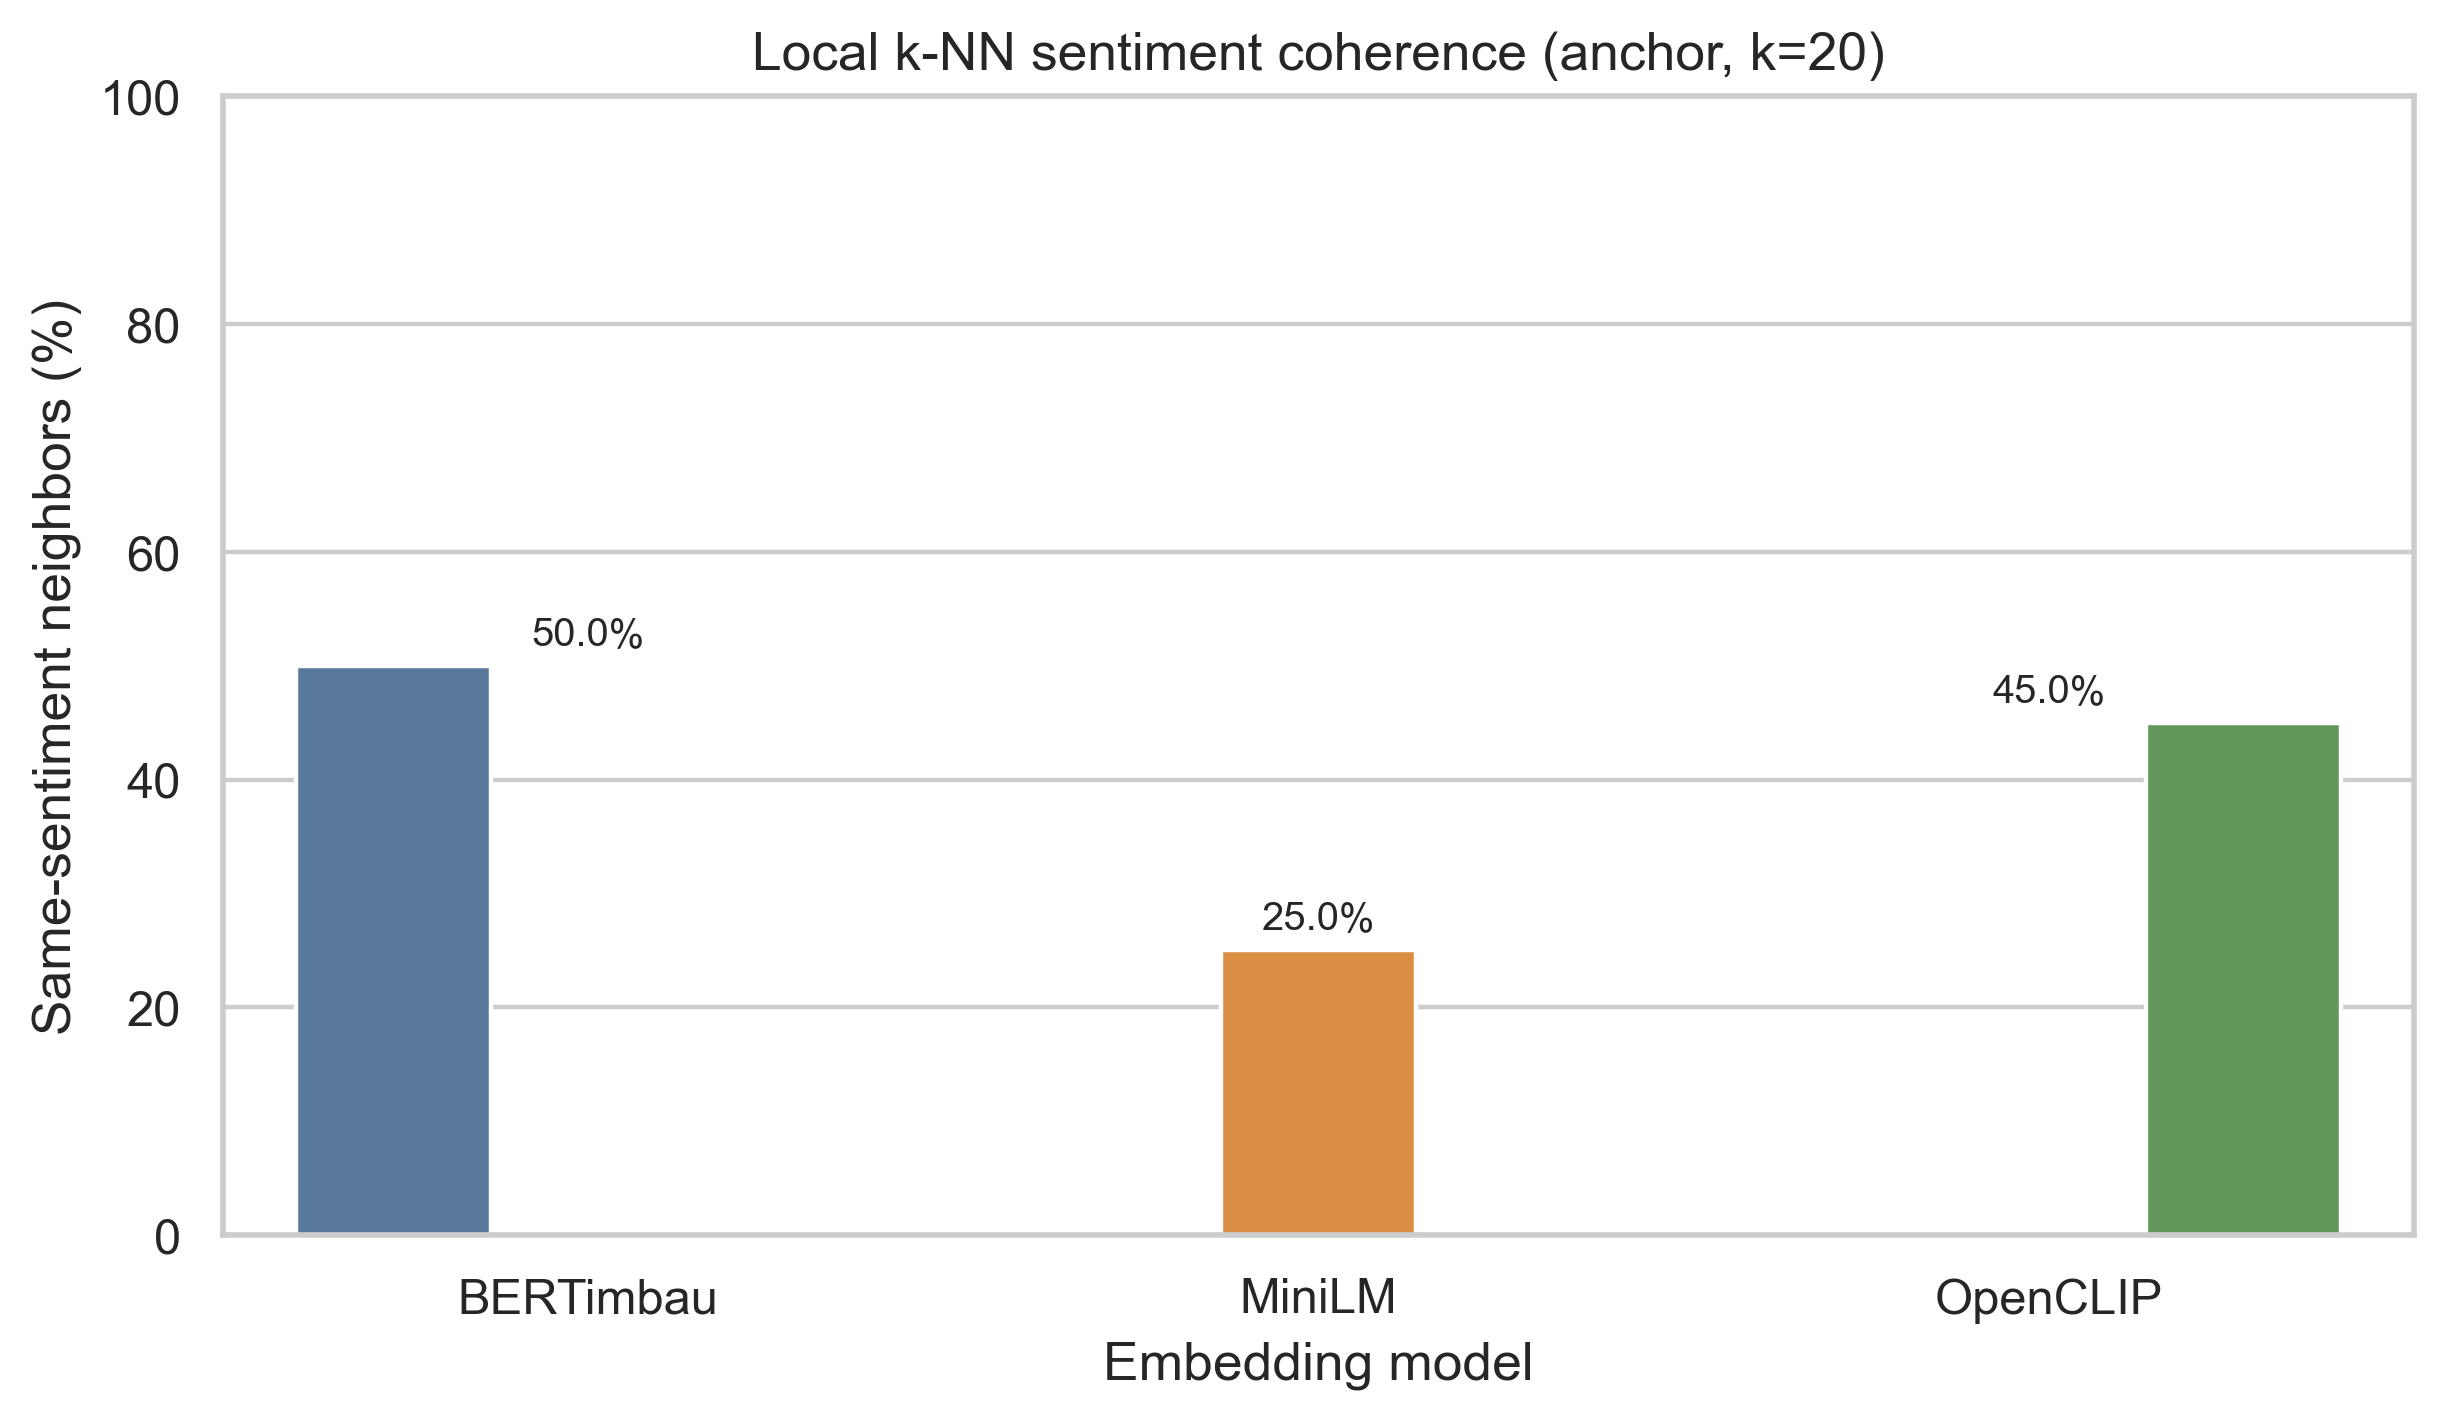
\includegraphics[width=\linewidth]{olist_negative_sentiment_geometry_assets/figures/phase3_knn_same_sentiment_share_k20.png}
\caption{Same-sentiment share among the 20 nearest neighbours for the ambiguous anchor across embedding models.}
\label{fig:knn-same-sentiment-share}
\end{figure}

For this anchor, the share of neighbours with the same sentiment as the anchor (positive) is 0.50 in BERTimbau, 0.25 in MiniLM, and 0.45 in OpenCLIP. 
Hence, all models preserve topical proximity around delivery/cancellation language, but they differ in local sentiment coherence: MiniLM is the most sentiment-mixed, BERTimbau is the most coherent for this case, and OpenCLIP is intermediate.

This focused diagnostic supports the broader islandisation analysis in Section~\ref{subsec:island-metrics} and Sections~5.5--5.6: local neighbourhood geometry is topic-consistent across models, while sentiment mixing varies by embedding family.

\section{Discussion and Limitations}
\label{sec:discussion}

This study asked whether negative reviews in Brazilian e-commerce form geometric ``islands'' or a diffuse layer in embedding space (RQ1), and how this behaviour varies across BERTimbau, Multilingual MiniLM, and OpenCLIP text encoders (RQ2). 
The results indicate a mixed picture: negative sentiment is neither uniformly spread nor confined to a single region, but instead concentrates in a small number of dense, sentiment-heavy clusters while also appearing in a more diffuse layer interwoven with broader service topics. 
Islandisation strength is clearly model-dependent, with BERTimbau and MiniLM exhibiting stronger negative concentration than OpenCLIP.
\subsection{Sentiment versus Topic Geometry}

The purity and projection analyses show that, given the simple regex-based topic proxy, clusters are more strongly aligned with sentiment than with topic in all three models. 
This suggests that even without explicit supervision, modern sentence embeddings tend to organise review texts along a polarity axis, with service dimensions such as delivery or product quality layered on top rather than forming fully separate clusters.

At the same time, the islandisation metrics reveal that negativity does not collapse into a single ``complaint cluster''. 
Instead, negative islands emerge around specific failure modes, such as non-delivery or incomplete orders, while other negatives are scattered across mixed clusters discussing delivery, product, and price. 
This pattern is consistent with recent work arguing that single-vector embeddings capture broad semantic axes but struggle to disentangle fine-grained factors such as sentiment and topic simultaneously.
\subsection{Model-dependent Islandisation}

The comparison across BERTimbau, MiniLM, and OpenCLIP suggests that training regime and model family materially affect how complaints are arranged in embedding space. 
MiniLM achieves the highest sentiment purity and relatively high negative homophily, indicating that it separates polarity well at the cluster level while still distributing negative reviews across several service themes rather than concentrating them in a single island.

BERTimbau, in contrast, tends to form tighter negative pockets: its negative homophily is strong and some clusters have very high negative ratios, which can be advantageous when the goal is to detect serious complaints but may under-represent milder or context-dependent negativity. 
OpenCLIP, trained for cross-modal alignment rather than solely textual semantics, shows weaker sentiment purity and homophily and higher dispersion for negatives, which aligns with its design as a more general, visually grounded encoder rather than a sentiment-focused model.

\subsection{Practical Implications}

From an applied perspective, the geometry-first workflow can support operational monitoring of customer complaints. 
First, negative-dense clusters can be tracked as early warning regions for recurring failures (for example, delivery delays or incomplete orders), such as a delivery-delay cluster whose negative share suddenly increases over a week. 
Second, local $k$-NN homophily around newly arriving negative reviews can surface similar complaints quickly, even without training a dedicated supervised classifier for each issue type. 
Third, because the cross-model comparison changes the observed island pattern, model choice should be treated as a business decision: tighter negative pockets (BERTimbau) may help triage severe incidents, while more diffuse coverage (MiniLM) may better capture distributed dissatisfaction.

\subsection{Limitations}

Several limitations qualify these findings. 
First, the primary sentiment signal is derived from star ratings, which are noisy and often reflect a combination of product, logistics, and platform experience; although the lexicon-based probe helps diagnose mismatches, it is itself imperfect and does not replace fine-grained human annotation. 
Second, the topic proxy is intentionally simple and regex-based, so topic purity estimates are conservative and likely underestimate the true topical structure of the corpus.

Third, all geometric analyses rely on single-vector sentence embeddings and cosine-based neighbourhoods; recent work has highlighted theoretical limits of such representations for capturing complex semantic structure, especially when multiple factors of variation must be encoded in a fixed-length vector. 
Fourth, the island definition uses heuristics (negative ratio thresholds and density) and is evaluated on a single dataset from a specific Brazilian marketplace context, so generalisation to other domains or languages remains an open question.

\clearpage
\section{Bibliography}
\printbibliography

\clearpage
\section*{}
\thispagestyle{empty}
\phantom{}

\end{document}
